\documentclass[a4paper, 12pt]{article}

%%%%%%%%%%%%
% Packages %
%%%%%%%%%%%%

\usepackage[french, english]{babel}

\usepackage[noheader]{packages/sleek}
\usepackage{packages/sleek-title}
\usepackage{packages/sleek-listings}
\usepackage{packages/sleek-theorems}

\usepackage{animate}

%%%%%%%%%%%%%%
% Title-page %
%%%%%%%%%%%%%%

\logo{resources/pdf/logo-uliege.pdf}
\institute{University of Liège}
%\faculty{}
%\department{}
\title{Assignment 2}
\subtitle{Optimal decision making for complex problems}
\author{%
Maxime \textsc{Meurisse} (s161278)\\%
François \textsc{Rozet} (s161024)%
}
%\supervisor{}
%\context{}
\date{Academic year 2020-2021}

%%%%%%%%%%%%%%%%
% Bibliography %
%%%%%%%%%%%%%%%%

\addbibresource{resources/bib/references.bib}

%%%%%%%%%%%%
% Document %
%%%%%%%%%%%%

\begin{document}
    \maketitle
    
    \section{Implementation of the Domain}
    
    We implement the different components of the \emph{car-on-the-hill} problem in the \texttt{domain.py} file.
    
    In this problem, the time is discretized, meaning that between two successive time steps $t$ and $t + 1$ a constant time $\Delta = \SI{0.1}{\second}$ passes. To implement the environment dynamics, we exploit the \emph{Euler integration method}. The integration step being $\delta = \SI{0.001}{\second}$, at each transition, we update the state by applying $\frac{\Delta}{\delta} = \num{100}$ times
    \begin{equation}
        x \gets x + \delta \dot{x}
    \end{equation}
    where $\dot{x}$ is equivalent to $(\dot{p}, \dot{s})$, defined in the statement. Our implementation handles the terminal states case by checking if either $\abs{p} > 1$ or $\abs{s} > 3$.
    
    \subsection{Rule-based policy}
    
    We called our rule-based policy the \enquote{step back policy} as the agent initially moves backward before accelerating to gain momentum in the downhill. Formally,
    \begin{equation}\label{eq:stepback.policy}
        \mu(p, s) = 4 \begin{cases}
            -1 & \text{if } \num{-0.5} < p < 0 \text{ and } \num{-1.5} < s < 0 \\
            +1 & \text{else}
        \end{cases}
    \end{equation}
    
    This policy is used to simulate a \emph{terminating} trajectory, starting at an initial state sampled from the distribution presented in the statement ($p_0 \sim \mathcal{U}(\num{-0.1}, \num{0.1})$ and $s_0 = 0$). This trajectory is illustrated in Listing \ref{lst:simulated.domain}.
    
    \begin{lstlisting}[style=defaultFrameTB, gobble=8, caption={A terminating trajectory of the policy \eqref{eq:stepback.policy}.}, label={lst:simulated.domain}]
        ((0.014, 0), 4, 0, (0.001, -0.290))
        ((0.001, -0.29), 4, 0, (-0.043, -0.592))
        ((-0.043, -0.592), -4, 0, (-0.141, -1.409))
        ((-0.141, -1.409), -4, 0, (-0.331, -2.415))
        ((-0.331, -2.415), 4, 0, (-0.572, -2.224))
        ((-0.572, -2.224), 4, 0, (-0.754, -1.389))
        ((-0.754, -1.389), 4, 0, (-0.852, -0.575))
        ((-0.852, -0.575), 4, 0, (-0.873, 0.16))
        ((-0.873, 0.16), 4, 0, (-0.82, 0.92))
        ((-0.82, 0.92), 4, 0, (-0.686, 1.778))
        ((-0.686, 1.778), 4, 0, (-0.47, 2.448))
        ((-0.47, 2.448), 4, 0, (-0.228, 2.247))
        ((-0.228, 2.247), 4, 0, (-0.031, 1.675))
        ((-0.031, 1.675), 4, 0, (0.118, 1.409))
        ((0.118, 1.409), 4, 0, (0.255, 1.348))
        ((0.255, 1.348), 4, 0, (0.391, 1.382))
        ((0.391, 1.382), 4, 0, (0.535, 1.514))
        ((0.535, 1.514), 4, 0, (0.697, 1.737))
        ((0.697, 1.737), 4, 0, (0.884, 2.028))
        ((0.884, 2.028), 4, 1, (1.104, 2.363))
    \end{lstlisting}
    
    \newpage
    
    \section{Expected Return of a Policy in Continuous Domain}\label{sec:expected.return}
    
    In the car-on-the-hill problem, the dynamics $f$ and reward signal $r$ of the environment are deterministic, \ie{} a state-action pair $(x, u)$ will always lead to the same one-step transition $(x, u, r, x')$. However, the choice of the initial state $x_0$ is stochastic. Therefore, the expected return $J^\mu$ of a policy $\mu$ can be expressed as
    \begin{equation}
        J^\mu = E_{x_0 \sim p(x_0)} \cbk{ \lim_{N \to \infty} \sum_{i = 0}^{N - 1} \gamma^i r(x_i, \mu(x_i)) }
    \end{equation}
    where $x_{i + 1} = f(x_i, \mu(x_i))$ and $\gamma \in [0; 1)$ is the discount factor. Interestingly, because $r$ is non-null only once in a trajectory, we have
    \begin{equation}
        \norm{J^\mu}_\infty \leq \norm{r}_\infty = B_r = 1 .
    \end{equation}
    In order to estimate the expected return, we have to fix a time horizon $N$ such that
    \begin{equation}\label{eq:N-expected.return}
        J^\mu_N = E_{x_0 \sim p(x_0)} \cbk{ \sum_{i = 0}^{N - 1} \gamma^i r(x_i, \mu(x_i)) }
    \end{equation}
    is a good approximation of $J^\mu$. In the car-on-the-hill environment, it can be shown \cite{ernstinfo8003, rozet2021suboptimality} that
    \begin{equation}
        \norm{J^\mu - J^\mu_N}_\infty \leq \gamma^N \norm{J^\mu} \leq \gamma^N B_r
    \end{equation}
    which can be used to enforce a certain precision. With a threshold $\epsilon = \num{e-2}$, we have
    \begin{align*}
        \gamma^N B_r & \leq \epsilon \\
        N & \geq \log_\gamma \frac{\epsilon}{B_r}
    \end{align*}
    which leads the smallest acceptable value
    \begin{equation}\label{eq:N-smallest.acceptable}
        N = \left\lceil \log_\gamma \frac{\epsilon}{B_r} \right\rceil = 90.
    \end{equation}
    Still, it is not possible to compute $J^\mu_N$ exactly as there is an infinite number of possible initial states $x_0$. Therefore, the expectation has to be approximated as well. This is done using the \emph{Monte Carlo} method, \ie{} approximating the expected return by the average cumulative reward over several trajectories. Let $h = (x_0, u_0, r_0, x_1, \dots, u_{t - 1}, r_{t - 1}, x_t)$ denote a trajectory of length $t$. Since $x_t$ can be the only terminal state of $h$, the cumulative reward $C_h$ is computed as
    \begin{equation}
        C_h = \sum_{i = 0}^{t - 1} \gamma^i r_i = \gamma^{t - 1} r_{t - 1} .
    \end{equation}
    Then, to estimate $J^\mu_N$, we simulate $n$ trajectories $h_i$ of length $N$ or less and compute
    \begin{equation}
        J^\mu_N \simeq \frac{1}{n} \sum_{i = 0}^{n - 1} C_{h_i} .
    \end{equation}
    We implement this as a routine and estimate the expected return of our policy \eqref{eq:stepback.policy} over $n = 50$ trajectories (truncated at $N$). The obtained values, from $1$ to $N$\footnote{With definition \eqref{eq:N-expected.return}, $J^\mu_0$ doesn't have a meaning.}, are shown in Figure \ref{fig:expected.return.monte.carlo}.
    
    \begin{figure}[H]
        \centering
        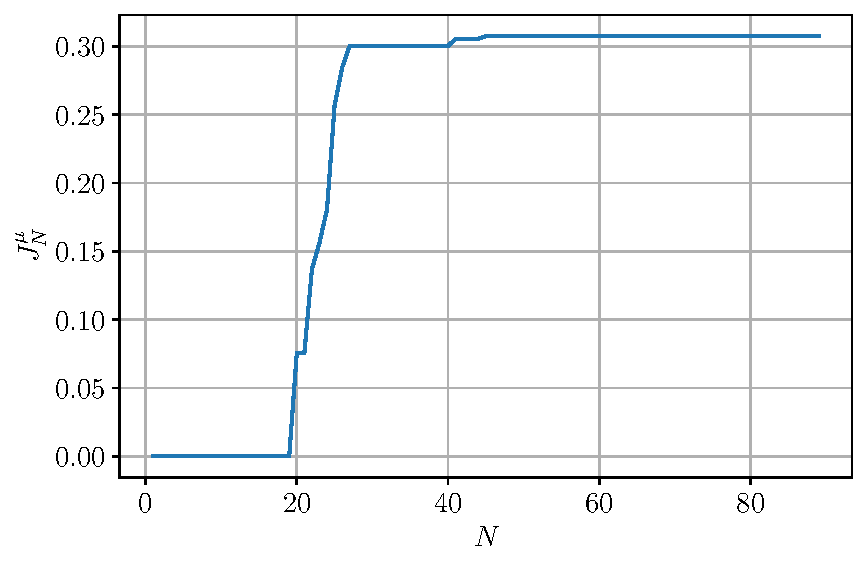
\includegraphics[width=0.7\textwidth]{resources/pdf/2_expected_return.pdf}
        \caption{$J^\mu_N$ of the policy \eqref{eq:stepback.policy} w.r.t. $N$.}
        \label{fig:expected.return.monte.carlo}
    \end{figure}
    
    One can see that the (approximated) expected return converged to a fixed value close to $\num{0.31}$ (with  a precision $\epsilon$).
    
    \section{Visualization}
    
    The visual rendering tools are implemented in the \texttt{display.py} file. Our routine is inspired from the Python script provided with the statement.
    
    We simulate the policy \eqref{eq:stepback.policy} starting at initial state $(p_0, s_0) = (0, 0)$ and produce a GIF file by assembling all output images produced. The latter, provided in the archive of our project, can also be visualized in Figure \ref{fig:stepback.policy.visualization}.
    
    \begin{figure}[H]
        \centering
        \animategraphics[autoplay, loop, width=0.4\textwidth]{10}{resources/png/stepback-}{1}{23}
        \caption{Visualization of the policy \eqref{eq:stepback.policy}, starting at initial state $(p_0, s_0) = (0, 0)$. \emph{This is an animated figure that is best viewed using Adobe Reader}.}
        \label{fig:stepback.policy.visualization}
    \end{figure}
    
    \section{Fitted-Q-Iteration}\label{sec:fqi}
    
    The goal of the \emph{Fitted-Q-Iteration} algorithm is to train a sequence of supervised regressors $\hat{Q}_1$, $\hat{Q}_2$, \dots, $\hat{Q}_N$ estimating respectively the functions $Q_1$, $Q_2$, \dots, $Q_N$. To do so, $N$ training sets are built. Let $h$ be an available set of $t$ one-step transitions $\cbk{(x_k, u_k, r_k, x'_k) \mid k = 1, \ldots, t}$. Then, the training sets are
    \begin{align*}
        \text{TS}_1 & = \cbk{\rbk{(x, u), r} \mid (x, u, r, x') \in h} \\
        \text{TS}_N & = \cbk{\rbk{(x, u), r + \gamma \max _{u' \in U} \hat{Q}_{N - 1}(x', u')} \mid (x, u, r, x') \in h } \quad \forall N \geq 2
    \end{align*}
    and $\hat{Q}_N$ is trained on $\text{TS}_N$. However, in the car-on-the-hill problem, one cannot take an action if the current state is terminal. Therefore, we tweak the formula as
    \begin{equation}
        \text{TS}_N = \cbk{\rbk{(x, u), r + I_{\cbk{r = 0}} \gamma \max _{u' \in U} \hat{Q}_{N - 1}(x', u')} \mid (x, u, r, x') \in h } \quad \forall N \geq 2
    \end{equation}
    where $I$ is the identity function.
    
    \subsection{Generation of $h$}\label{sec:h.generation}
    
    We implement two generation strategies code-named \enquote{Exhaustive} and \enquote{Monte Carlo}, respectively.
    
    \begin{description}
        \item[Exhaustive] The first generation strategy is inspired by the \enquote{exhaustive grid search} hyperparameter optimization technique. We cut the state space into $200 \times 200$ uniformly spaced grid cells $x_{ij} = (p_i, s_j)$ and apply all possible actions $u$ (\num{+4} or \num{-4}) to them.
        \begin{equation}
            h = \cbk{\rbk{x_{ij}, u, r(x_{ij}, u), f(x_{ij}, u)} \mid 1 \leq i, j \leq 200, u \in U}
        \end{equation}
        
        The main advantage of this strategy is that the state space is very well covered. Especially, edge cases are represented. However, a drawback is that the distribution of state-action pairs is not similar to those of trajectories. Therefore, a lot of pairs could be useless (unreachable) and confuse the supervised algorithm.
        
        \item[Monte Carlo] The second strategy is simply to simulate $n$ trajectories $h_i$ with a uniform random policy starting from a random ($p_0 \sim \mathcal{U}(\num{-0.1}, \num{0.1})$ and $s_0 = 0$) initial state $x_0$ and to aggregate them as a single set.
        \begin{equation}
            h = \bigcup_{i=0}^{n - 1} h_i
        \end{equation}
        
        In practice, we don't choose $n$; we simulate trajectories of at most \num{1000} transitions until the total number of transitions is \num{80000}, \ie{} the same number of transitions than the exhaustive strategy.
        
        The advantages/drawbacks of this strategy are the opposite of the previous one: the state space is unlikely to be well covered but the distribution should correspond better to those of actual trajectories.        
    \end{description}
    
    \subsection{Stopping rules}\label{sec:stopping.rules}
    
    We thought of two stopping rules.
    
    \begin{enumerate}
        \item As in Section \ref{sec:expected.return}, for the car-on-the-hill problem, it can be shown \cite{ernstinfo8003, rozet2021suboptimality} that
            \begin{equation}
                \norm{J^{\mu^*} - J^{\mu^*_N}}_\infty \leq \frac{2 \gamma^N}{1 - \gamma} \norm{J^\mu} \leq \frac{2 \gamma^N}{1 - \gamma} B_r .
            \end{equation}
            Our first rule is to choose $N$ such that the suboptimality of $\mu^*_N$ is bounded by $\epsilon = \num{e-2}$, which is achieved with
            \begin{equation}
                N = \left\lceil \log_{\gamma} \rbk{\frac{\epsilon}{2 B_r}(1-\gamma)} \right\rceil = \num{162} .
            \end{equation}
        \item The second idea is to stop the FQI algorithm when the estimators' predictions have or seemed to have \enquote{converged}, \ie{} we want
        \begin{equation}
            \norm{\hat{Q}_N - \hat{Q}_{N - 1}}_\infty \leq \epsilon
        \end{equation}
        with $\epsilon$ arbitrarily set to $0.02$. However, in the continuous domain it is not possible to compute exactly this infinite norm. Instead, we replace it by a mean absolute difference
        \begin{equation}\label{eq:mad}
            \frac{1}{2 t} \sum_{(x, u, r, x') \in h, u' \in U} \abs{\hat{Q}_N(x', u') - \hat{Q}_{N-1}(x', u')}
        \end{equation}
        which allows to \enquote{reuse} quantities computed during the creation of $\text{TS}_N$ and $\text{TS}_{N+1}$.
    \end{enumerate}
    
    \subsection{Supervised algorithms}\label{sec:supervised.algorithms}
    
    As requested by the statement, we implement 3 supervised algorithms:
    
    \begin{enumerate}
        \item Linear Regression, borrowed as-is from \texttt{scikit-learn};
        \item Extremely Randomized Trees, also borrowed from \texttt{scikit-learn} but with \enquote{only} 20 estimators;
        \item Neural Network, implemented using \texttt{tensorflow.keras}. As architecture, we chose a simple \emph{Multi-Layer Perceptron} (MLP) with 3 hidden layers of 8 neurons each and ReLU activation functions. The inputs are $(p, s, u)$ triples and the outputs are $\hat{Q}_N((p, s), u)$ scalars. This architecture is represented in Figure \ref{fig:mlp.architecture}.
        \begin{figure}[H]
    	    \centering
    	    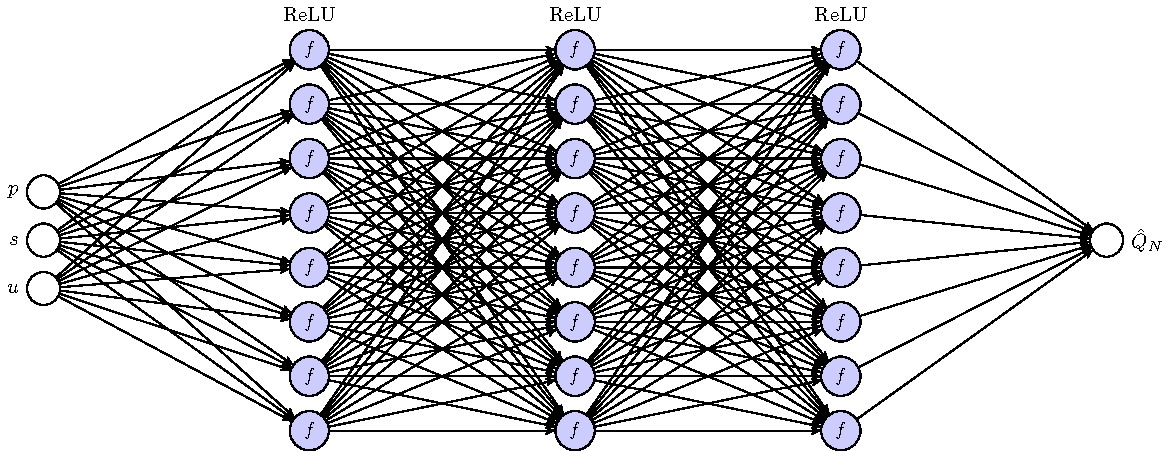
\includegraphics[width=0.9\textwidth]{resources/tikz/nn.pdf}
    	    \caption{Architecture of the MLP used in the Fitted-Q-Iteration algorithm.}
    	    \label{fig:mlp.architecture}
    	\end{figure}
    	The network is trained using the Adam \cite{kingma2014adam} optimizer with the \emph{Mean Squared Error} (MSE) loss. This architecture is relatively narrow and shallow. The reason behind this choice is that the size(s) of our training set(s) is relatively moderate and the number of inputs is very small. Consequently, if we were to increase the width and/or depth of our network, the network could end-up overfitting the training data. In fact, restricting the width/depth of a neural network is a kind of \emph{regularization} as it reduces the model's expressivity, which usually helps to \emph{generalize}. The same goes for the number of estimators and maximal depth of Randomized Trees.
    \end{enumerate}
    
    We train these supervised algorithms, for all (4) combinations of generation strategy and stopping rule, using the FQI algorithm. We then use them to estimate the state-action values $Q_N(x, u)$ on a uniformly spaced (resolution of \num{0.01}) grid of the state space for all possible actions.
    
    In the following, the state-action values are displayed on separate figures for each action. A third figure is used to display the policy $\hat{\mu}^*_N$ inferred from $\hat{Q}_N$ as
    \begin{equation}\label{eq:mu.derived}
        \hat{\mu}^*_N(x) \in \arg\max_{u \in U} Q(x, u) .
    \end{equation}
    The action $-4$ is represented in red and the action $+4$ in blue.
    
    We then estimate the expected return $J^{\hat{\mu}^*_N}$ of the policy, using the routines implemented for Section \ref{sec:expected.return}. It should be noted that we truncate the sampled trajectories to $N' = 90$ transitions, according to relation \eqref{eq:N-smallest.acceptable}.
    
    \blindfootnote{For the sake of conciseness, we chose to display the figures in $2 \times 2$ grids, which necessarily reduces the size of the figures and labels. However, the plots are \emph{vectorized}, which implies that, in the digital document, the font will stay crisp at any level of zoom.}
    
    \newpage
    
    \subsubsection{Linear Regression}
    
    \begin{figure}[H]
        \centering
        \begin{subfigure}{0.49\textwidth}
            \centering
            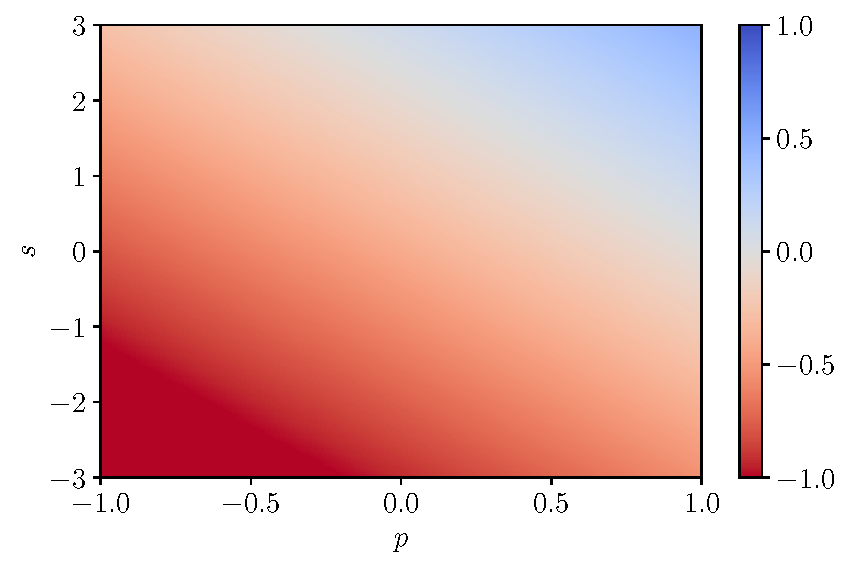
\includegraphics[width=0.85\textwidth]{resources/pdf/4_exhaustive_1_LR_q_-4.pdf}
            \caption{Exhaustive, stopping rule 1; $N = 162$.}
            \vspace{0.5em}
        \end{subfigure}
        \hfill
        \begin{subfigure}{0.49\textwidth}
            \centering
            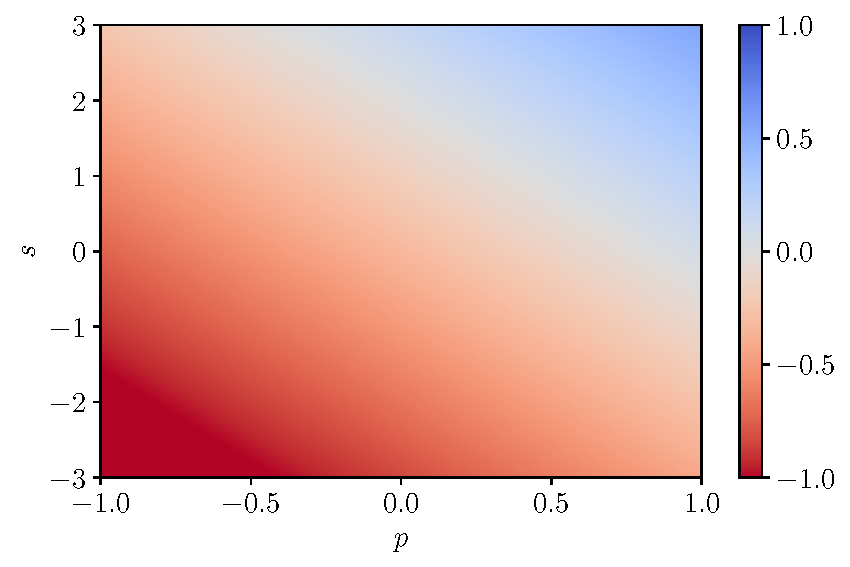
\includegraphics[width=0.85\textwidth]{resources/pdf/4_exhaustive_2_LR_q_-4.pdf}
            \caption{Exhaustive, stopping rule 2; $N = 7$.}
            \vspace{0.5em}
        \end{subfigure}
        \begin{subfigure}{0.49\textwidth}
            \centering
            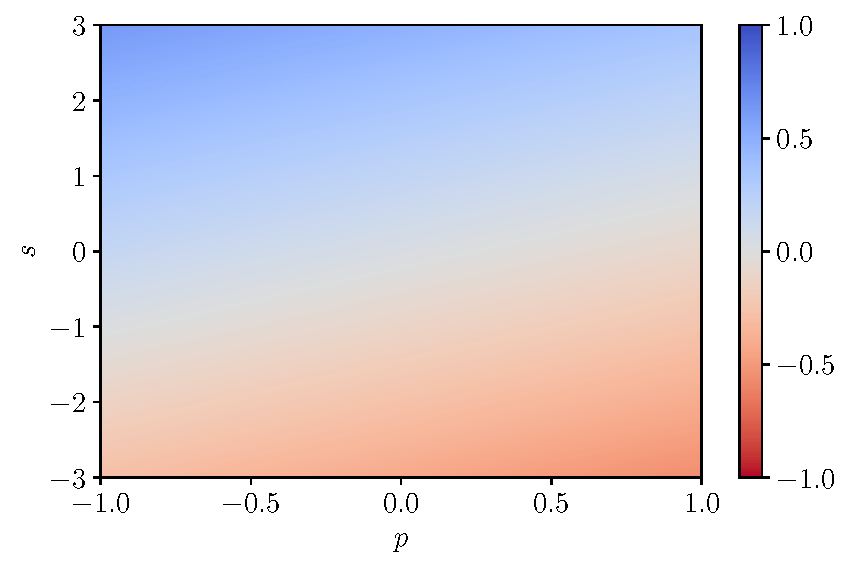
\includegraphics[width=0.85\textwidth]{resources/pdf/4_montecarlo_1_LR_q_-4.pdf}
            \caption{Monte Carlo, stopping rule 1; $N = 162$.}
        \end{subfigure}
        \hfill
        \begin{subfigure}{0.49\textwidth}
            \centering
            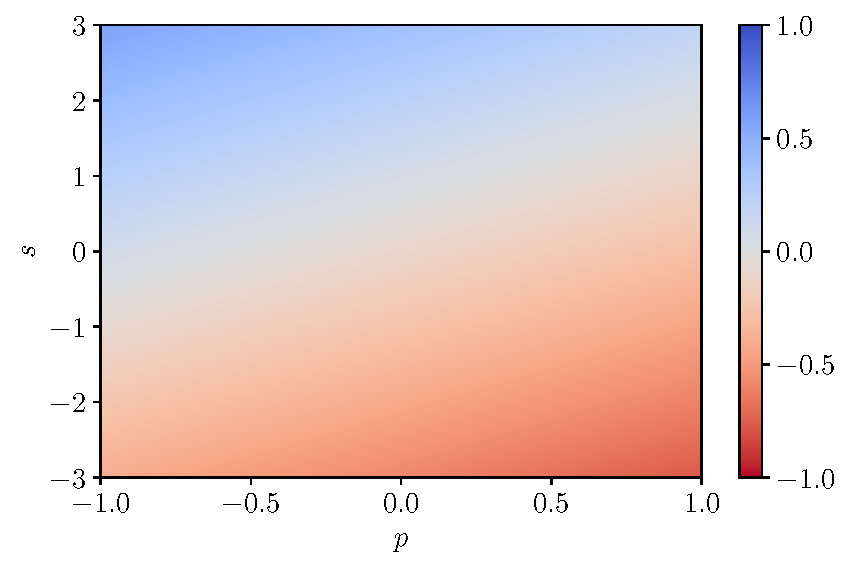
\includegraphics[width=0.85\textwidth]{resources/pdf/4_montecarlo_2_LR_q_-4.pdf}
            \caption{Monte Carlo, stopping rule 2; $N = 10$.}
        \end{subfigure}
        \noskipcaption{$\hat{Q}_N((p, s), -4)$ values of the Linear Regression algorithm.}
        \label{fig:qn.lr.minus.4}
    \end{figure}
    
    \begin{figure}[H]
        \centering
        \begin{subfigure}{0.49\textwidth}
            \centering
            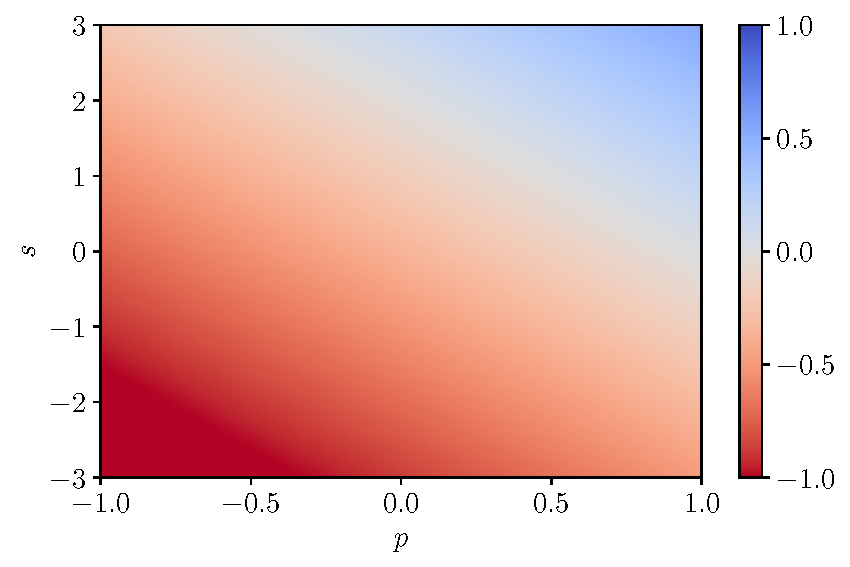
\includegraphics[width=0.85\textwidth]{resources/pdf/4_exhaustive_1_LR_q_+4.pdf}
            \caption{Exhaustive, stopping rule 1; $N = 162$.}
            \vspace{0.5em}
        \end{subfigure}
        \hfill
        \begin{subfigure}{0.49\textwidth}
            \centering
            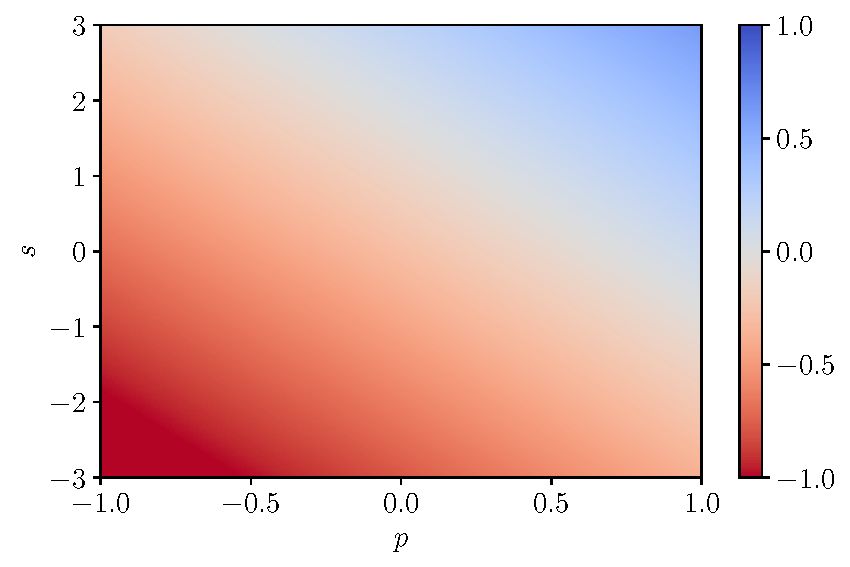
\includegraphics[width=0.85\textwidth]{resources/pdf/4_exhaustive_2_LR_q_+4.pdf}
            \caption{Exhaustive, stopping rule 2; $N = 7$.}
            \vspace{0.5em}
        \end{subfigure}
        \begin{subfigure}{0.49\textwidth}
            \centering
            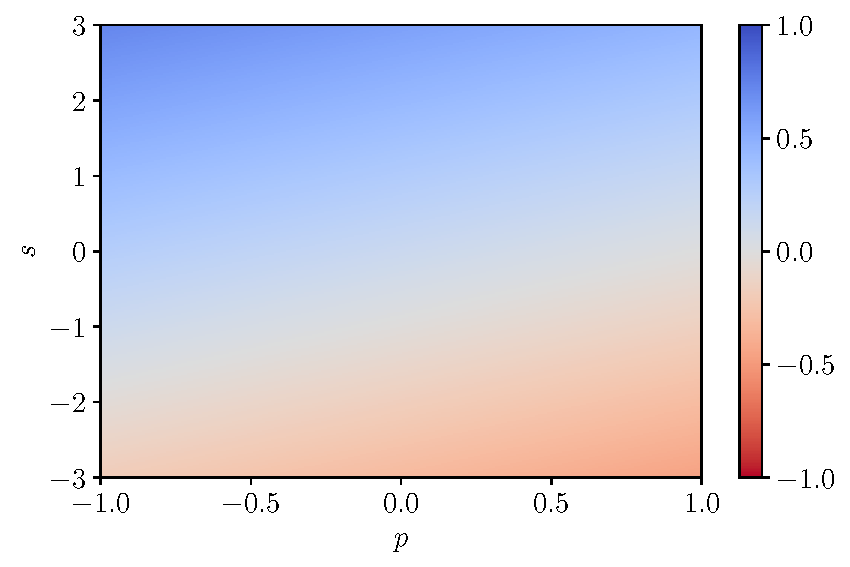
\includegraphics[width=0.85\textwidth]{resources/pdf/4_montecarlo_1_LR_q_+4.pdf}
            \caption{Monte Carlo, stopping rule 1; $N = 162$.}
        \end{subfigure}
        \hfill
        \begin{subfigure}{0.49\textwidth}
            \centering
            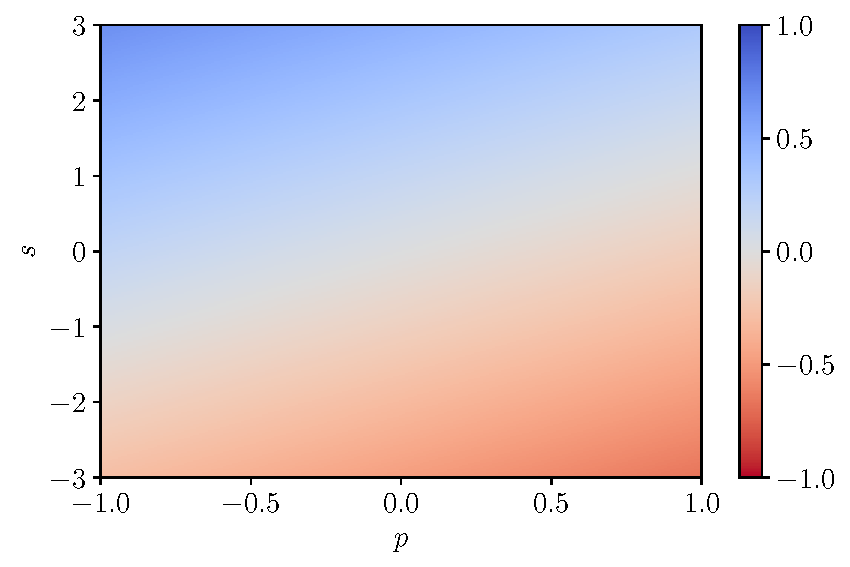
\includegraphics[width=0.85\textwidth]{resources/pdf/4_montecarlo_2_LR_q_+4.pdf}
            \caption{Monte Carlo, stopping rule 2; $N = 10$.}
        \end{subfigure}
        \noskipcaption{$\hat{Q}_N((p, s), +4)$ values for the Linear Regression algorithm.}
        \label{fig:qn.lr.plus.4}
    \end{figure}
    
    \begin{figure}[H]
        \centering
        \begin{subfigure}{0.49\textwidth}
            \centering
            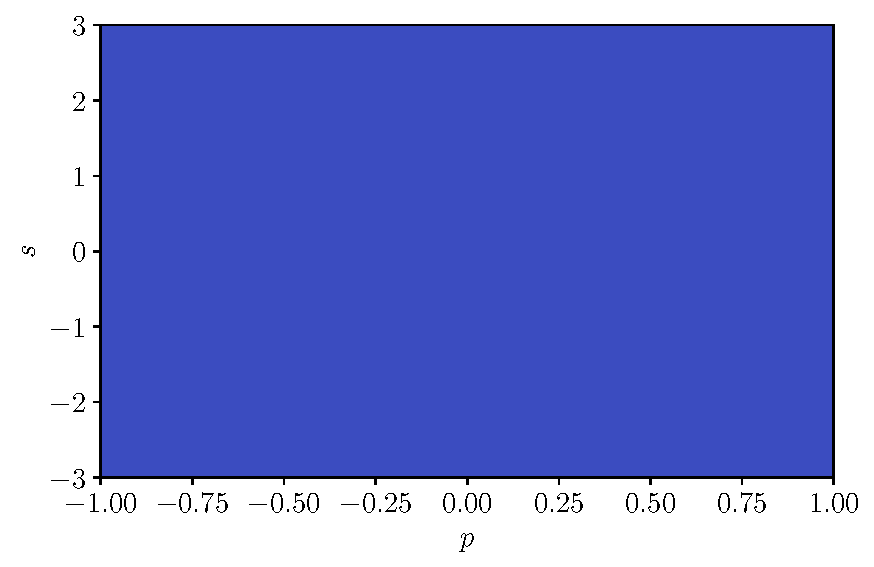
\includegraphics[width=0.85\textwidth]{resources/pdf/4_exhaustive_1_LR_mu.pdf}
            \caption{Exhaustive, stopping rule 1; $N = 162$.}
            \vspace{0.5em}
        \end{subfigure}
        \hfill
        \begin{subfigure}{0.49\textwidth}
            \centering
            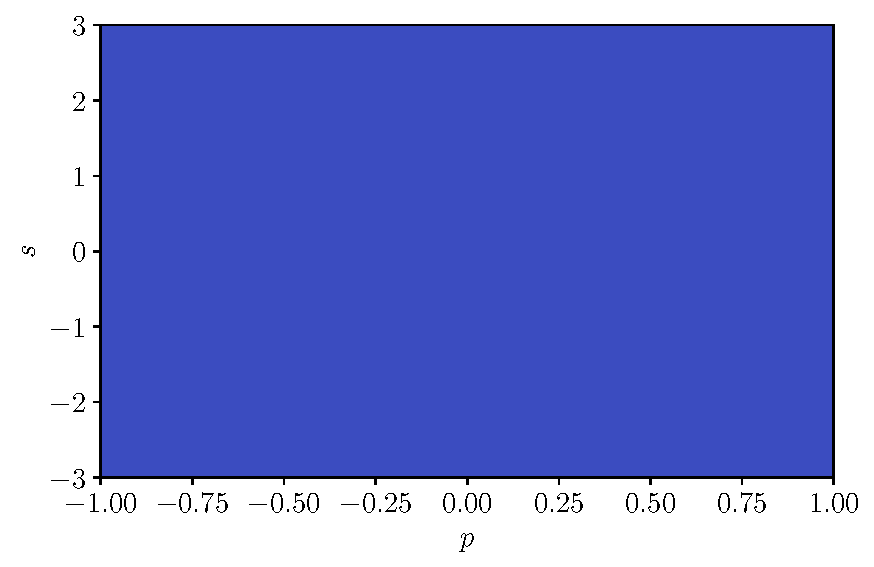
\includegraphics[width=0.85\textwidth]{resources/pdf/4_exhaustive_2_LR_mu.pdf}
            \caption{Exhaustive, stopping rule 2; $N = 7$.}
            \vspace{0.5em}
        \end{subfigure}
        \begin{subfigure}{0.49\textwidth}
            \centering
            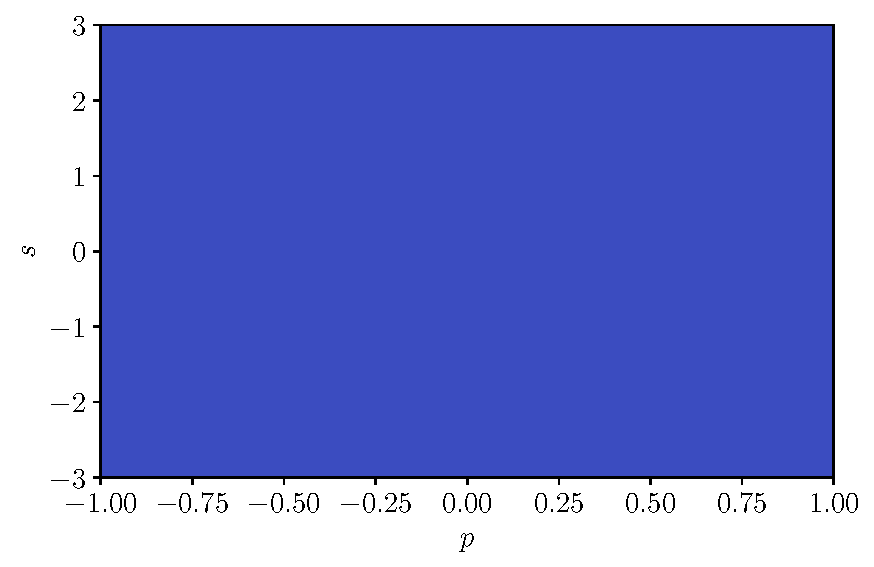
\includegraphics[width=0.85\textwidth]{resources/pdf/4_montecarlo_1_LR_mu.pdf}
            \caption{Monte Carlo, stopping rule 1; $N = 162$.}
        \end{subfigure}
        \hfill
        \begin{subfigure}{0.49\textwidth}
            \centering
            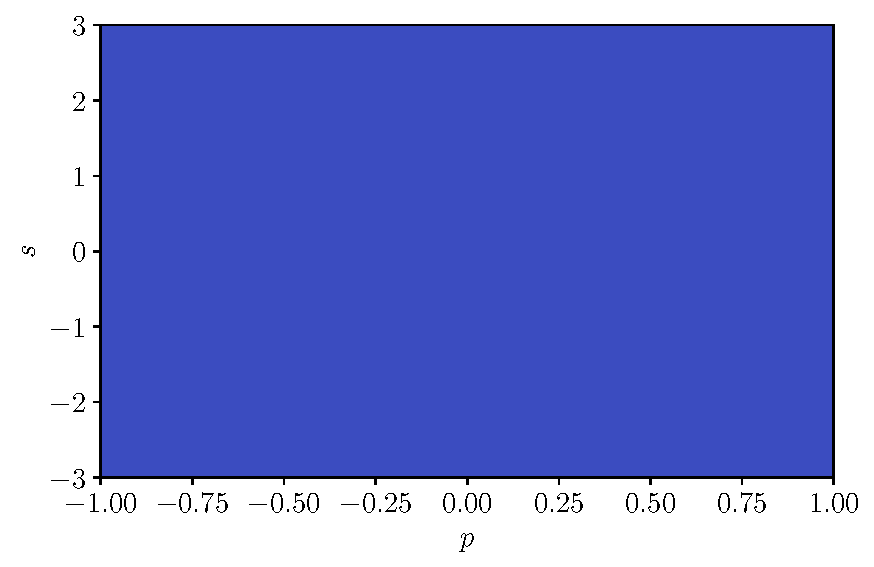
\includegraphics[width=0.85\textwidth]{resources/pdf/4_montecarlo_2_LR_mu.pdf}
            \caption{Monte Carlo, stopping rule 2; $N = 10$.}
        \end{subfigure}
        \caption{$\hat{\mu}_{N}^{*}$ policies inferred from the Linear Regression algorithm.}
        \label{fig:mu.lr}
    \end{figure}
    
    \begin{table}[H]
        \centering
        \begin{tabular}{c|c|c}
            & Stopping rule 1 & Stopping rule 2 \\
            \hline
            Exhaustive & \num{0.0} & \num{0.0} \\
            Monte Carlo & \num{0.0} & \num{0.0} \\
        \end{tabular}
        \caption{Estimations of the expected returns of $\hat{\mu}^*_N$.}
        \label{tab:expected.return.mu.lr}
    \end{table}
    
    \newpage
    
    \subsubsection{Extremely Randomized Trees}
    
    \begin{figure}[H]
        \centering
        \begin{subfigure}{0.49\textwidth}
            \centering
            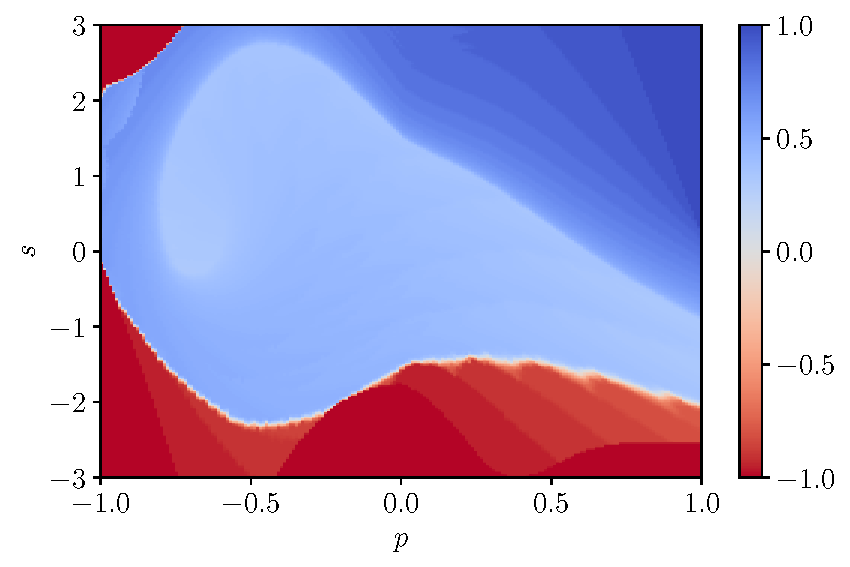
\includegraphics[width=0.85\textwidth]{resources/pdf/4_exhaustive_1_XRT_q_-4.pdf}
            \caption{Exhaustive, stopping rule 1; $N = 162$.}
            \vspace{0.5em}
        \end{subfigure}
        \hfill
        \begin{subfigure}{0.49\textwidth}
            \centering
            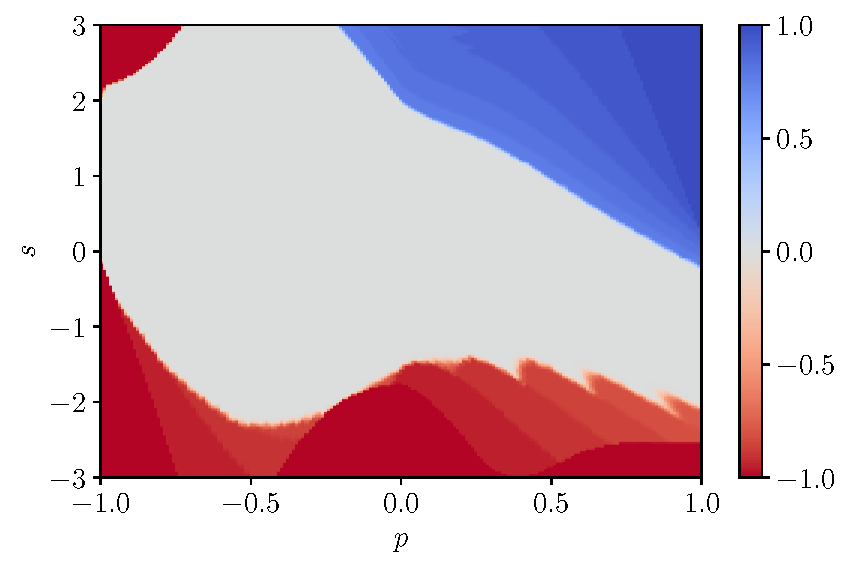
\includegraphics[width=0.85\textwidth]{resources/pdf/4_exhaustive_2_XRT_q_-4.pdf}
            \caption{Exhaustive, stopping rule 2; $N = 6$.}
            \vspace{0.5em}
        \end{subfigure}
        \begin{subfigure}{0.49\textwidth}
            \centering
            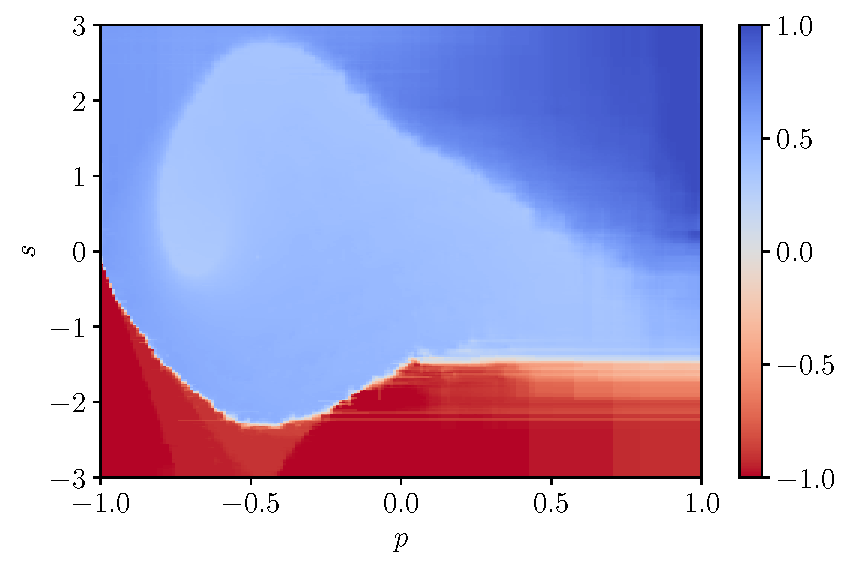
\includegraphics[width=0.85\textwidth]{resources/pdf/4_montecarlo_1_XRT_q_-4.pdf}
            \caption{Monte Carlo, stopping rule 1; $N = 162$.}
        \end{subfigure}
        \hfill
        \begin{subfigure}{0.49\textwidth}
            \centering
            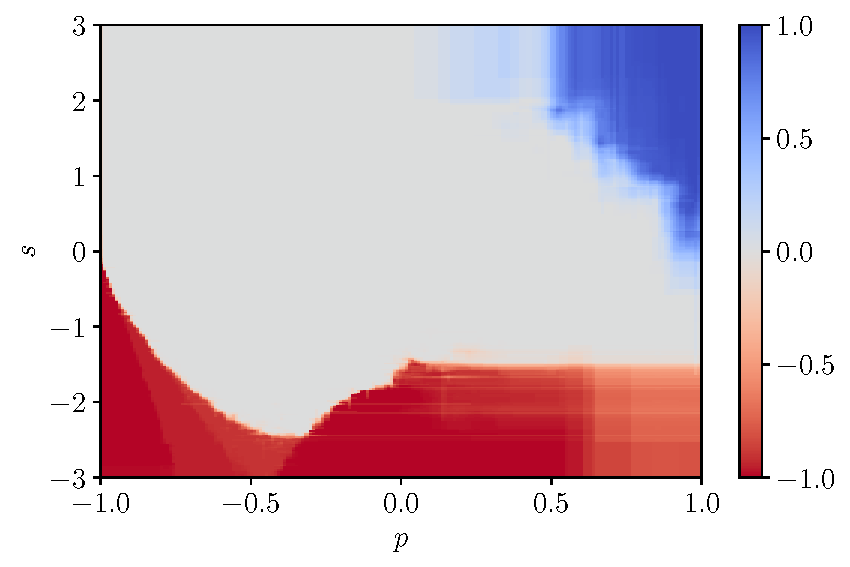
\includegraphics[width=0.85\textwidth]{resources/pdf/4_montecarlo_2_XRT_q_-4.pdf}
            \caption{Monte Carlo, stopping rule 2; $N = 3$.}
        \end{subfigure}
        \noskipcaption{$\hat{Q}_N((p, s), -4)$ values for the Extremely Randomized Trees algorithm.}
        \label{fig:qn.xrt.minus.4}
    \end{figure}
    
    \begin{figure}[H]
        \centering
        \begin{subfigure}{0.49\textwidth}
            \centering
            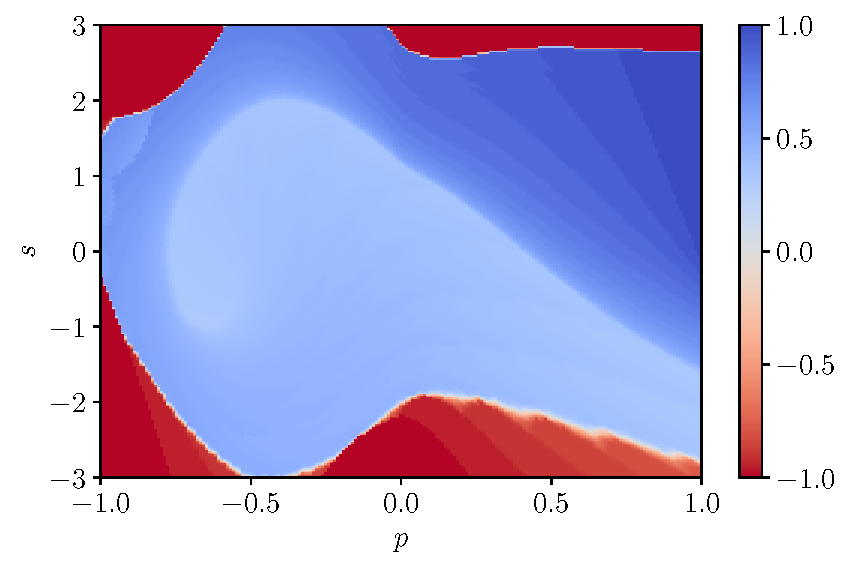
\includegraphics[width=0.85\textwidth]{resources/pdf/4_exhaustive_1_XRT_q_+4.pdf}
            \caption{Exhaustive, stopping rule 1; $N = 162$.}
            \vspace{0.5em}
        \end{subfigure}
        \hfill
        \begin{subfigure}{0.49\textwidth}
            \centering
            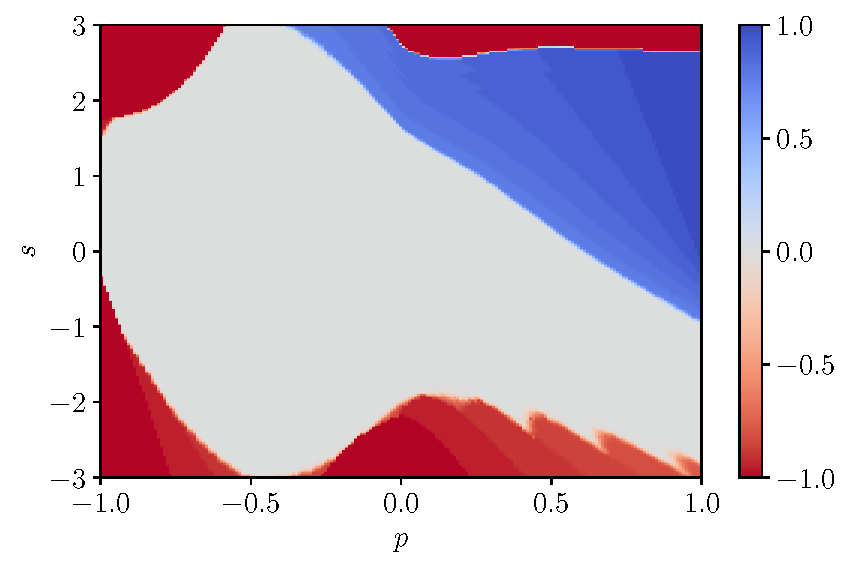
\includegraphics[width=0.85\textwidth]{resources/pdf/4_exhaustive_2_XRT_q_+4.pdf}
            \caption{Exhaustive, stopping rule 2; $N = 6$.}
            \vspace{0.5em}
        \end{subfigure}
        \begin{subfigure}{0.49\textwidth}
            \centering
            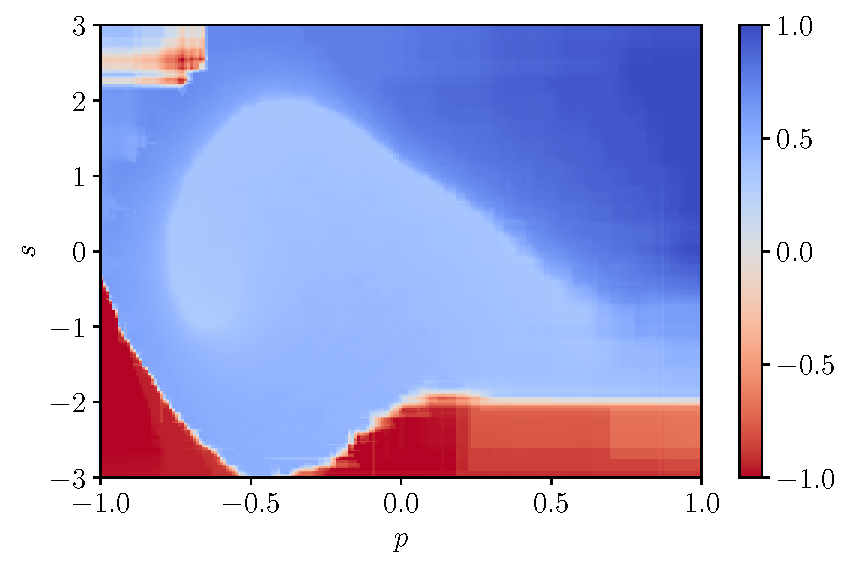
\includegraphics[width=0.85\textwidth]{resources/pdf/4_montecarlo_1_XRT_q_+4.pdf}
            \caption{Monte Carlo, stopping rule 1; $N = 162$.}
        \end{subfigure}
        \hfill
        \begin{subfigure}{0.49\textwidth}
            \centering
            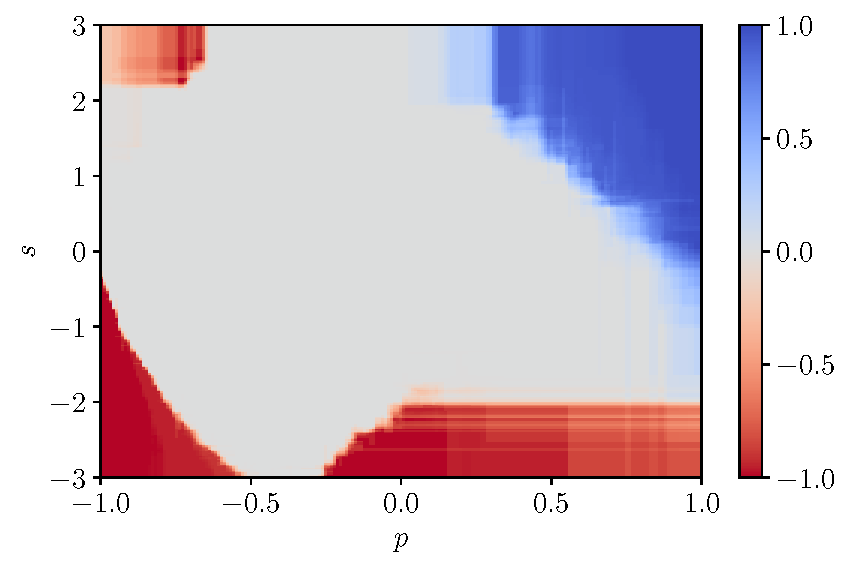
\includegraphics[width=0.85\textwidth]{resources/pdf/4_montecarlo_2_XRT_q_+4.pdf}
            \caption{Monte Carlo, stopping rule 2; $N = 3$.}
        \end{subfigure}
        \noskipcaption{$\hat{Q}_N((p, s), +4)$ values for the Extremely Randomized Trees algorithm.}
        \label{fig:qn.xrt.plus.4}
    \end{figure}
    
    \begin{figure}[H]
        \centering
        \begin{subfigure}{0.49\textwidth}
            \centering
            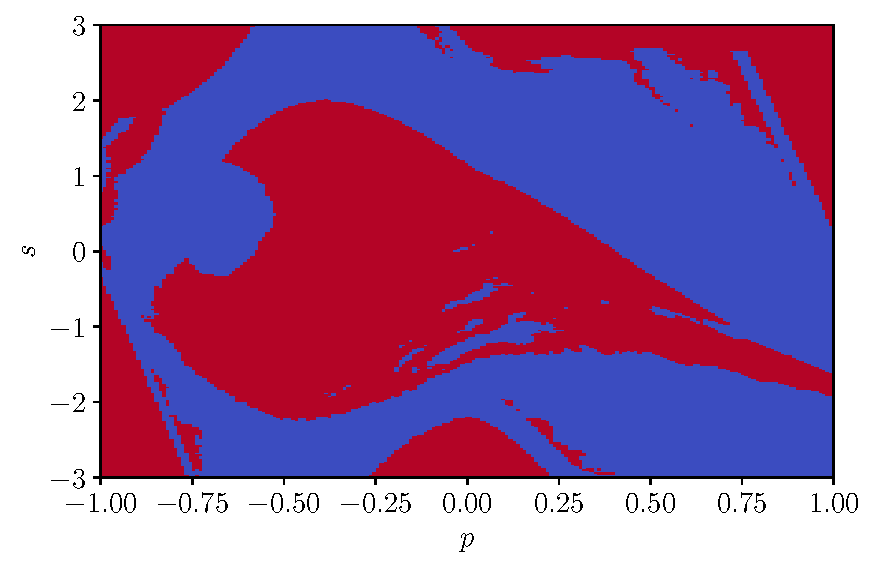
\includegraphics[width=0.85\textwidth]{resources/pdf/4_exhaustive_1_XRT_mu.pdf}
            \caption{Exhaustive, stopping rule 1; $N = 162$.}
            \vspace{0.5em}
        \end{subfigure}
        \hfill
        \begin{subfigure}{0.49\textwidth}
            \centering
            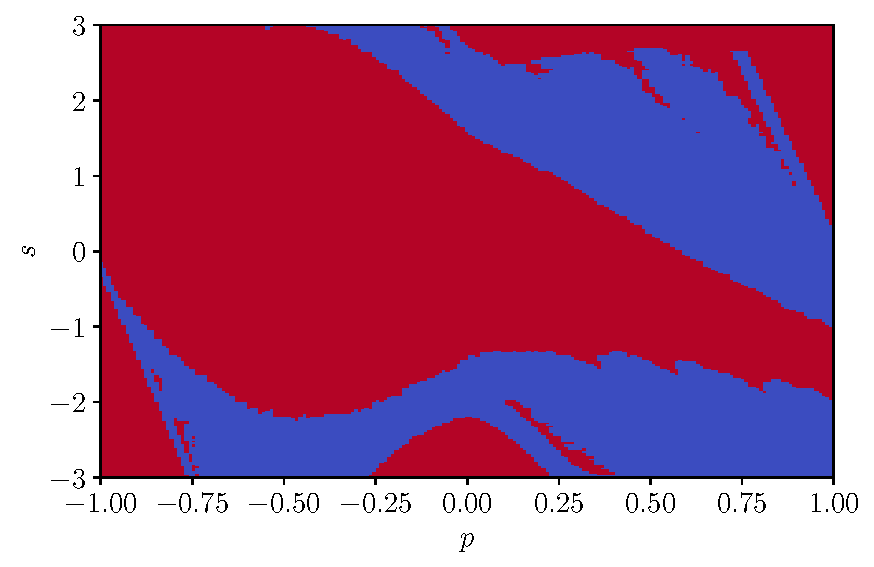
\includegraphics[width=0.85\textwidth]{resources/pdf/4_exhaustive_2_XRT_mu.pdf}
            \caption{Exhaustive, stopping rule 2; $N = 6$.}
            \vspace{0.5em}
        \end{subfigure}
        \begin{subfigure}{0.49\textwidth}
            \centering
            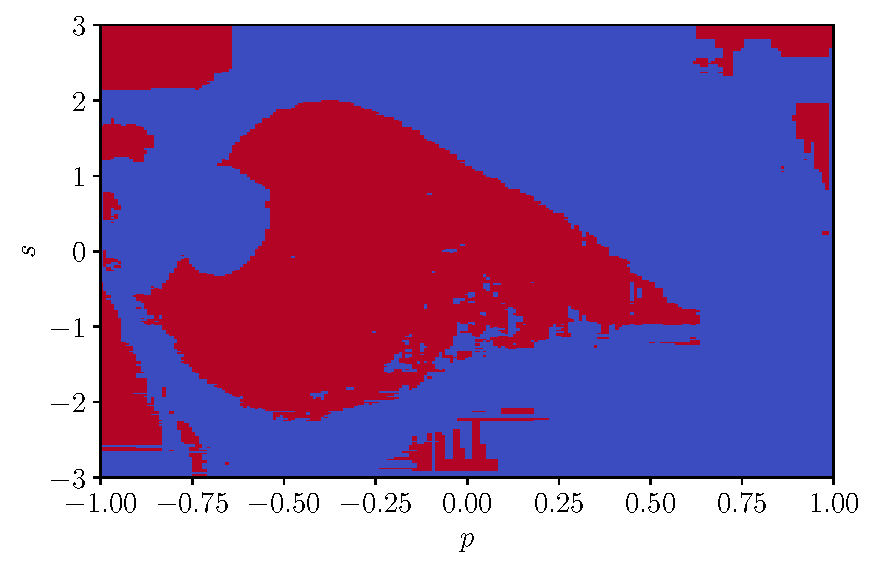
\includegraphics[width=0.85\textwidth]{resources/pdf/4_montecarlo_1_XRT_mu.pdf}
            \caption{Monte Carlo, stopping rule 1; $N = 162$.}
        \end{subfigure}
        \hfill
        \begin{subfigure}{0.49\textwidth}
            \centering
            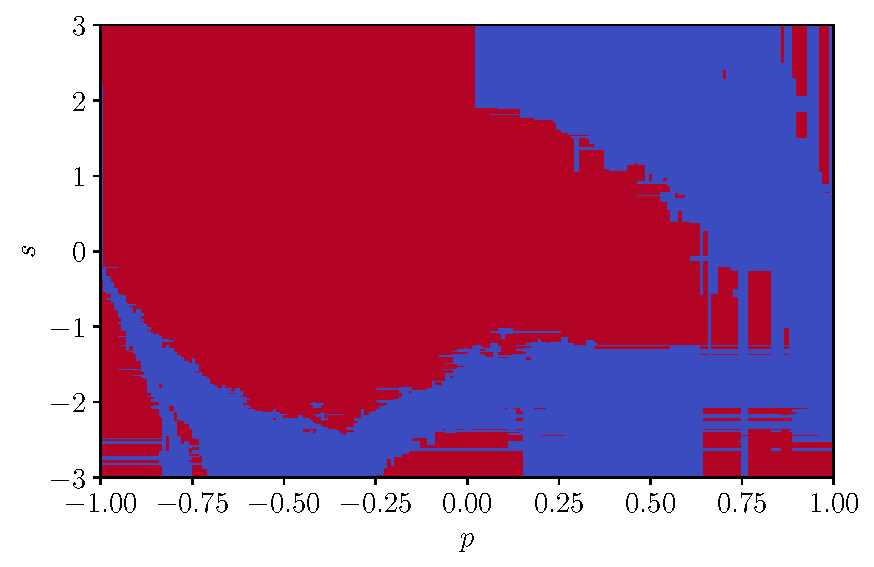
\includegraphics[width=0.85\textwidth]{resources/pdf/4_montecarlo_2_XRT_mu.pdf}
            \caption{Monte Carlo, stopping rule 2; $N = 3$.}
        \end{subfigure}
        \caption{$\hat{\mu}_{N}^{*}$ policies inferred from the Extremely Randomized Trees algorithm.}
        \label{fig:mu.xrt}
    \end{figure}
    
    \begin{table}[H]
        \centering
        \begin{tabular}{c|c|c}
            & Stopping rule 1 & Stopping rule 2 \\
            \hline
            Exhaustive & \num{0.42} & \num{0.0} \\
            Monte Carlo & \num{0.42} & \num{0.0} \\
        \end{tabular}
        \caption{Estimations of the expected returns of $\hat{\mu}^*_N$.}
        \label{tab:expected.return.mu.xrt}
    \end{table}
    
    \newpage
    
    \subsubsection{Neural Network}
	
	\begin{figure}[H]
	    \centering
        \begin{subfigure}{0.49\textwidth}
            \centering
            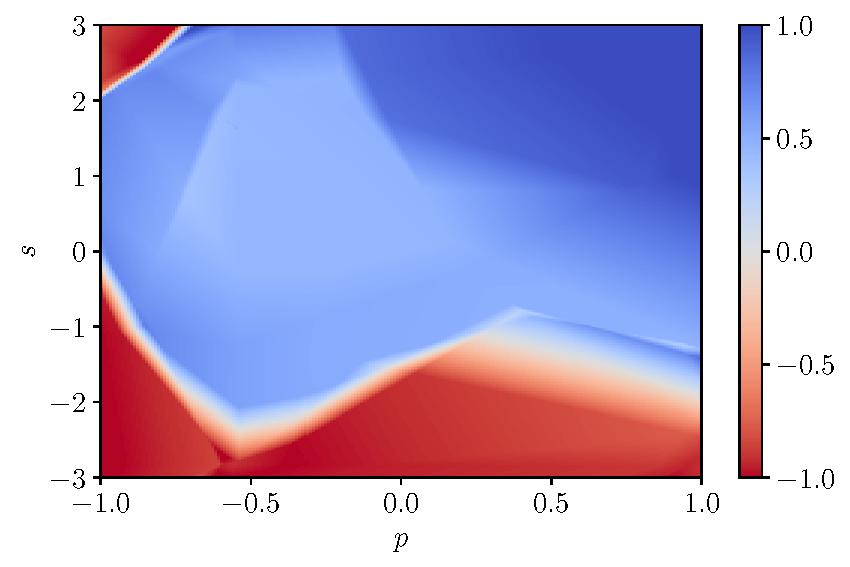
\includegraphics[width=0.85\textwidth]{resources/pdf/4_exhaustive_1_MLP_q_-4.pdf}
            \caption{Exhaustive, stopping rule 1; $N = 162$.}
            \vspace{0.5em}
        \end{subfigure}
        \hfill
        \begin{subfigure}{0.49\textwidth}
            \centering
            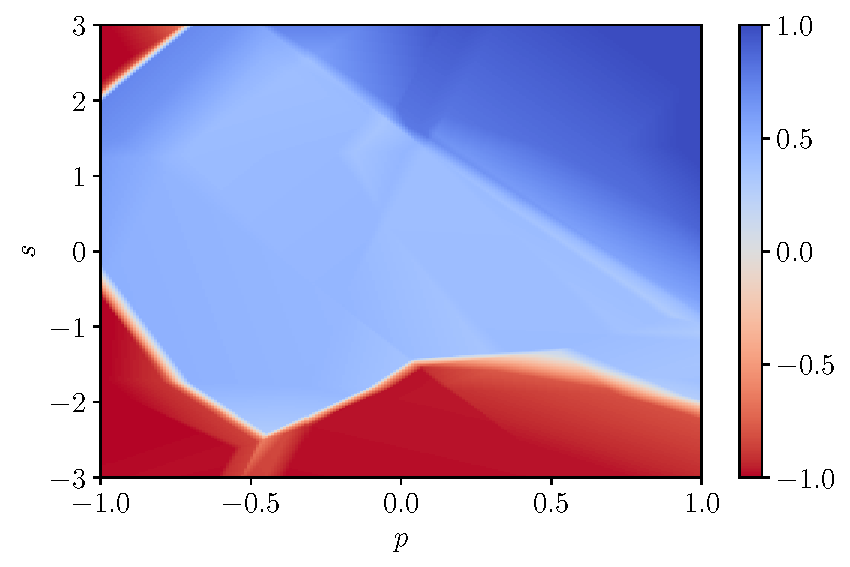
\includegraphics[width=0.85\textwidth]{resources/pdf/4_exhaustive_2_MLP_q_-4.pdf}
            \caption{Exhaustive, stopping rule 2; $N = 196$.}
            \vspace{0.5em}
        \end{subfigure}
        \begin{subfigure}{0.49\textwidth}
            \centering
            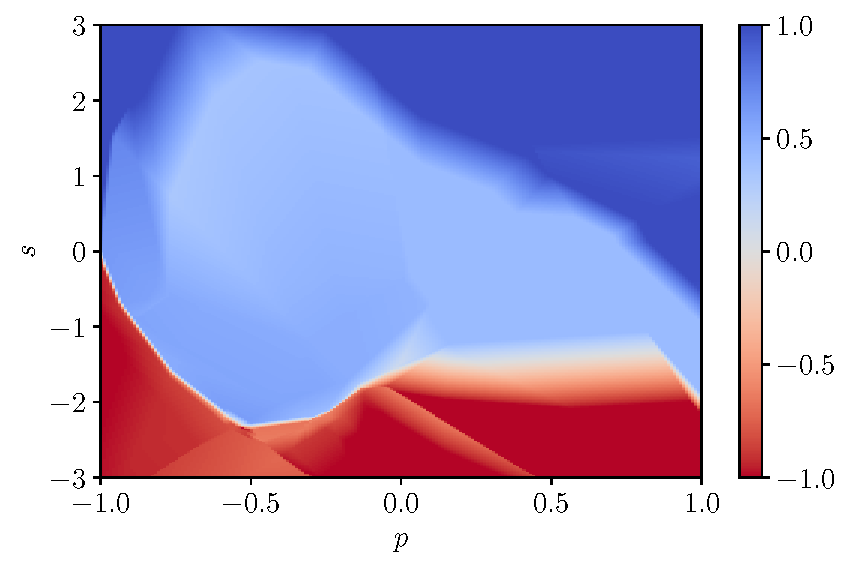
\includegraphics[width=0.85\textwidth]{resources/pdf/4_montecarlo_1_MLP_q_-4.pdf}
            \caption{Monte Carlo, stopping rule 1; $N = 162$.}
        \end{subfigure}
        \hfill
        \begin{subfigure}{0.49\textwidth}
            \centering
            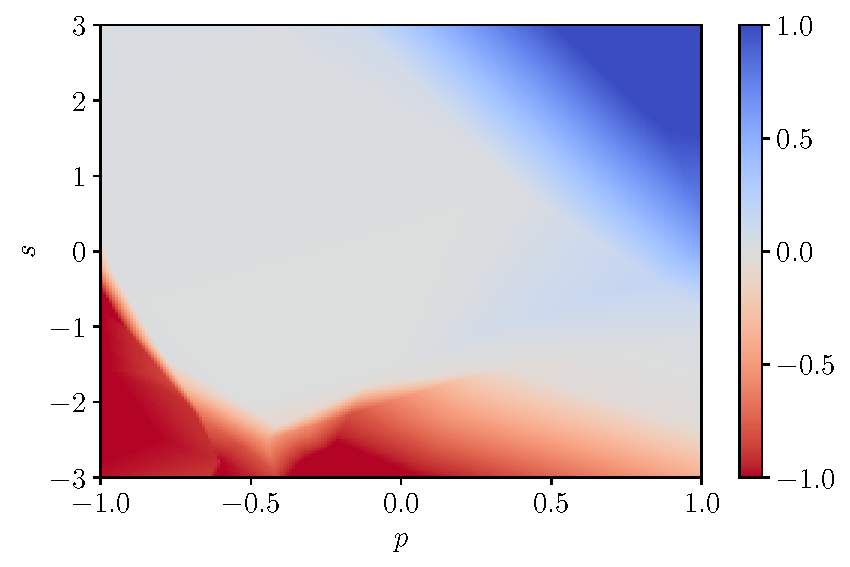
\includegraphics[width=0.85\textwidth]{resources/pdf/4_montecarlo_2_MLP_q_-4.pdf}
            \caption{Monte Carlo, stopping rule 2; $N = 5$.}
        \end{subfigure}
        \noskipcaption{$\hat{Q}_N((p, s), -4)$ values for the MLP algorithm.}
        \label{fig:qn.mlp.minus.4}
    \end{figure}
    
    \begin{figure}[H]
        \centering
        \begin{subfigure}{0.49\textwidth}
            \centering
            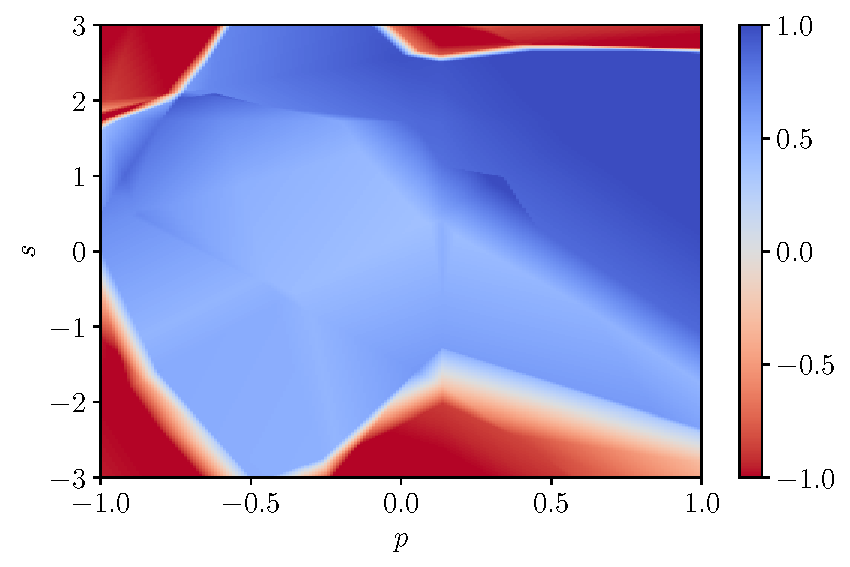
\includegraphics[width=0.85\textwidth]{resources/pdf/4_exhaustive_1_MLP_q_+4.pdf}
            \caption{Exhaustive, stopping rule 1; $N = 162$.}
            \vspace{0.5em}
        \end{subfigure}
        \hfill
        \begin{subfigure}{0.49\textwidth}
            \centering
            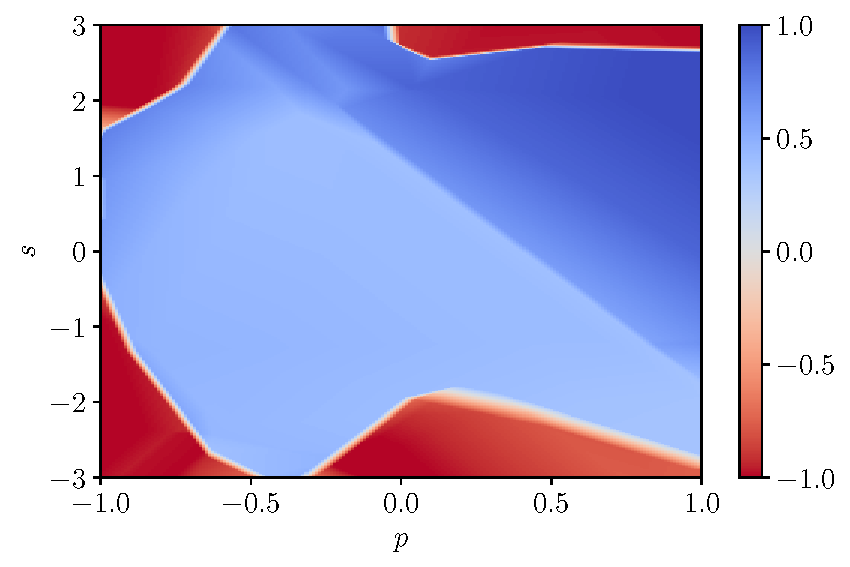
\includegraphics[width=0.85\textwidth]{resources/pdf/4_exhaustive_2_MLP_q_+4.pdf}
            \caption{Exhaustive, stopping rule 2; $N = 196$.}
            \vspace{0.5em}
        \end{subfigure}
        \begin{subfigure}{0.49\textwidth}
            \centering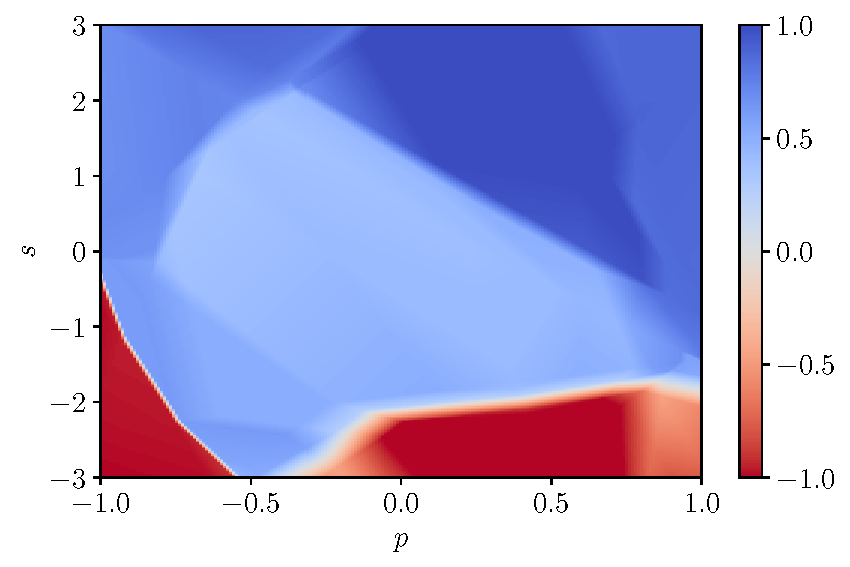
\includegraphics[width=0.85\textwidth]{resources/pdf/4_montecarlo_1_MLP_q_+4.pdf}
            \caption{Monte Carlo, stopping rule 1; $N = 162$.}
        \end{subfigure}
        \hfill
        \begin{subfigure}{0.49\textwidth}
            \centering
            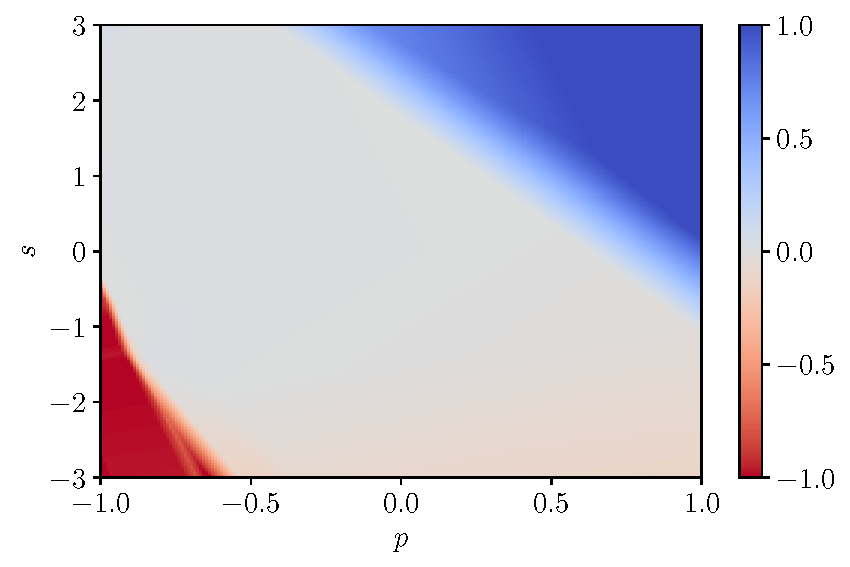
\includegraphics[width=0.85\textwidth]{resources/pdf/4_montecarlo_2_MLP_q_+4.pdf}
            \caption{Monte Carlo, stopping rule 2; $N = 5$.}
        \end{subfigure}
        \noskipcaption{$\hat{Q}_N((p, s), +4)$ values for the MLP algorithm.}
        \label{fig:qn.mlp.plus.4}
    \end{figure}
    
    \begin{figure}[H]
        \centering
        \begin{subfigure}{0.49\textwidth}
            \centering
            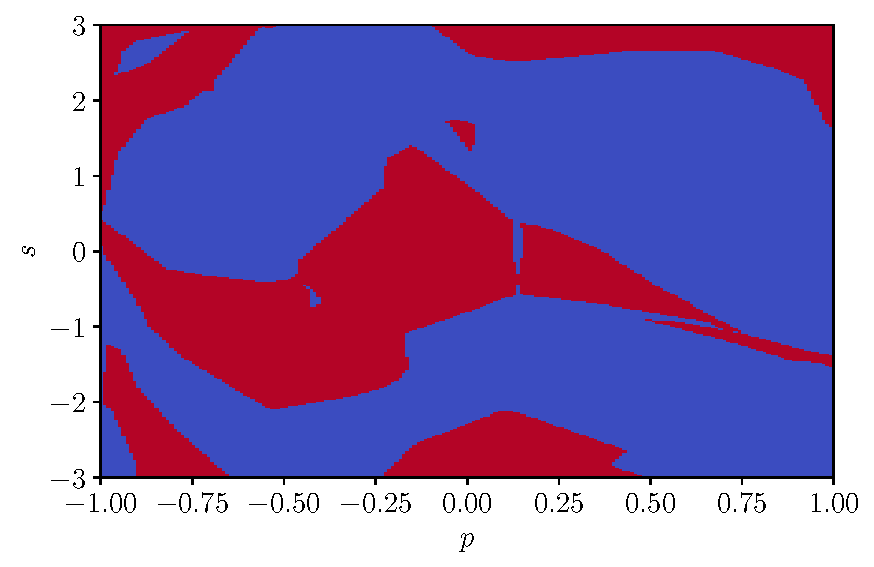
\includegraphics[width=0.85\textwidth]{resources/pdf/4_exhaustive_1_MLP_mu.pdf}
            \caption{Exhaustive, stopping rule 1; $N = 162$.}
            \vspace{0.5em}
        \end{subfigure}
        \hfill
        \begin{subfigure}{0.49\textwidth}
            \centering
            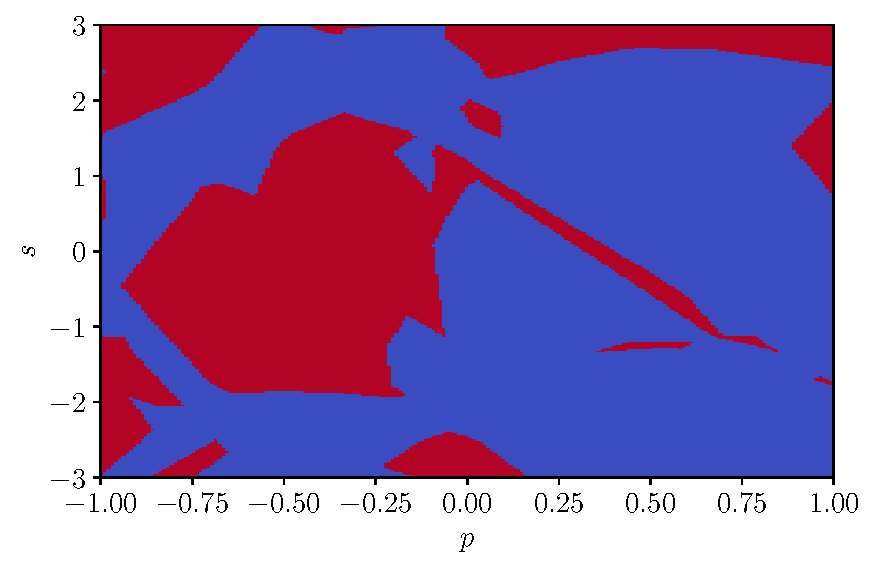
\includegraphics[width=0.85\textwidth]{resources/pdf/4_exhaustive_2_MLP_mu.pdf}
            \caption{Exhaustive, stopping rule 2; $N = 196$.}
            \vspace{0.5em}
        \end{subfigure}
        \begin{subfigure}{0.49\textwidth}
            \centering
            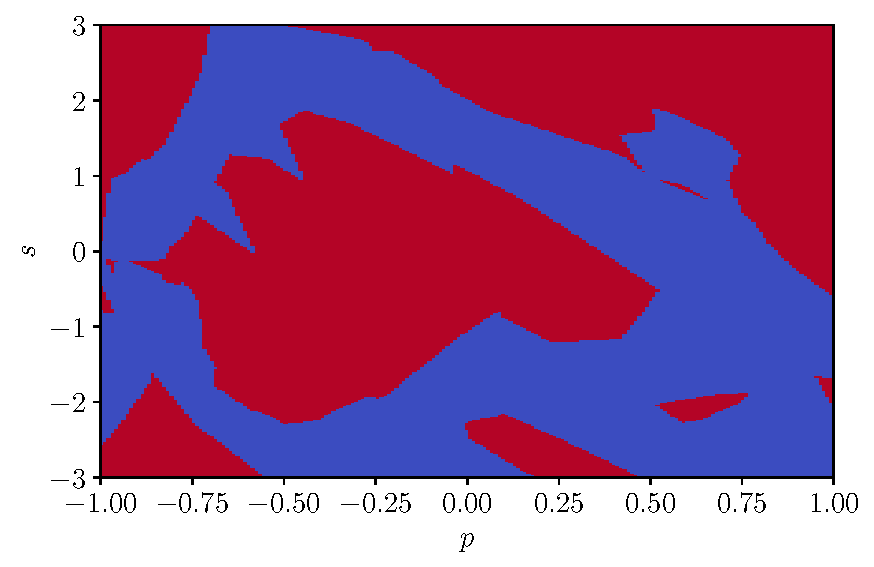
\includegraphics[width=0.85\textwidth]{resources/pdf/4_montecarlo_1_MLP_mu.pdf}
            \caption{Monte Carlo, stopping rule 1; $N = 162$.}
        \end{subfigure}
        \hfill
        \begin{subfigure}{0.49\textwidth}
            \centering
            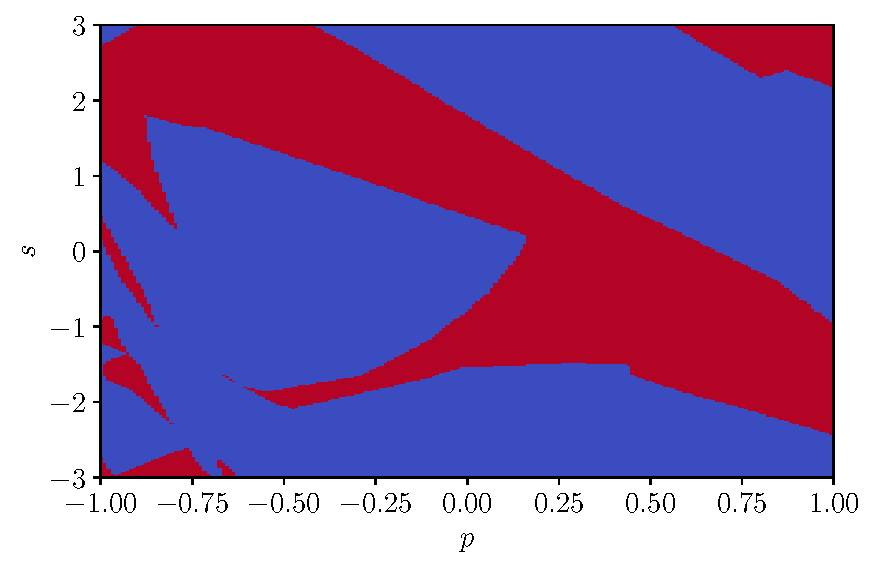
\includegraphics[width=0.85\textwidth]{resources/pdf/4_montecarlo_2_MLP_mu.pdf}
            \caption{Monte Carlo, stopping rule 2; $N = 5$.}
        \end{subfigure}
        \caption{$\hat{\mu}_{N}^{*}$ policies inferred from the MLP algorithm.}
        \label{fig:mu.mlp}
    \end{figure}
    
    \begin{table}[H]
        \centering
        \begin{tabular}{c|c|c}
            & Stopping rule 1 & Stopping rule 2 \\
            \hline
            Exhaustive & \num{0.38} & \num{0.35} \\
            Monte Carlo & \num{0.24} & \num{0.0} \\
        \end{tabular}
        \caption{Estimations of the expected returns of $\hat{\mu}^*_N$.}
        \label{tab:expected.return.mu.mlp}
    \end{table}
    
    \subsection{Discussion}
    
    In general, we observe that the results of the Linear Regression are terrible, those of the Extremely Randomized Trees are great and those with the MLP are in between.

    Concerning the Linear Regression, all combinations of generation strategy and stopping rule give the same policy: the agent systematically performs the action $u = +4$ (\cf{} Figure \ref{fig:mu.lr}). This might reflect that the model is only able to learn that, in general, the agent must go to the right. Indeed, by accelerating only to the right, the agent has a chance of getting a positive reward, whereas by accelerating only to the left, the agent is sure to never be able to win. Unfortunately this policy does not allow the agent to obtain rewards in a reasonable time, hence the null expected rewards.
    
    For Extremely Randomized Trees, the estimated $\hat{Q}_N$ values, for the stopping rule 1, seem very accurate. Indeed, we can see (\cf{} Figures \ref{fig:qn.xrt.minus.4} and \ref{fig:qn.xrt.plus.4}) that the estimator learned quite well were accelerating forward or backward makes you lose immediately, mainly because of the speed limit. For example, if you have a high positive speed at the top of the right hill, it is dangerous to accelerate forward. Interestingly, we observe that these \enquote{danger zones} are not as well defined for the Monte Carlo generation strategy. This is explained by the fact that it is not possible to be in that position with that much speed starting from the initial state. Therefore, even if the policies inferred with each generation strategy are slightly different, their are equivalent in practice and have the same expected return (\cf{} Table \ref{tab:expected.return.mu.xrt}), which is higher than the one of our step back policy \eqref{eq:stepback.policy}.
    
    For the stopping rule 2, the estimator is agnostic for a big part of the state-action space. This is explained by the fact that the FQI algorithm was stopped very early and before convergence. In fact, the threshold imposed on the mean absolute difference \eqref{eq:mad} does not ensure convergence afterwards. A more valid criterion would have been to wait for a \emph{plateau} of the mean absolute difference, \ie{} a long period during which the mean absolute difference doesn't change significantly.
    
    Finally, concerning the MLP, we notice that the $\hat{Q}_N$ values (\cf{} Figures \ref{fig:qn.mlp.minus.4} and \ref{fig:qn.mlp.plus.4}) are similar in sign to those of the Extremely Randomized Trees. However, their amplitudes are a little off, especially for the Monte Carlo generation strategy, which causes the inferred policy to be less effective and have a lower expected return (\cf{} Table \ref{tab:expected.return.mu.mlp}).
    
    For the exhaustive generation strategy and stopping rule 2, the FQI algorithm was stopped after $N = 196$ iterations. This is probably due to luck as it is very different with the Monte Carlo generation strategy ($N = 5$). Nevertheless, we observe that the $\hat{Q}_N$ values are actually closer to those of the Extremely Randomized Trees algorithm, which indicates that our MLP could profit from more FQI iterations.
    
    \newpage
    
    \section{Parametric Q-Learning}\label{sec:parametric.q.learning}
    
    As shown in the previous assignment, the \emph{Q-learning algorithm} allows us to directly infer $\hat{Q}$ from a set (not necessarily finite) of one-step transitions $h = \cbk{(x_k, u_k, r_k, x'_k) \mid k = 1, \ldots, t}$.
    
    We can \cite{ernstinfo8003} extend this algorithm to the case where a parametric $Q$-function estimator of the form $\hat{Q}(x, u, a)$ is used (\cf{} Algorithm \ref{alg:parametric.q.learning}).
    
    \begin{fmd-algorithm}[Parametric Q-learning (PQL)]\label{alg:parametric.q.learning}
        \begin{enumerate}
            \item Initialize $\hat{Q}(x, u, a)$ to $0$ everywhere.
            \item Until some stopping criterion, update the parameters following
            \begin{equation}\label{eq:parametric.update}
                a \gets a + \alpha \delta(x, u, r, x') \frac{\partial \hat{Q}(x, u, a)}{\partial a}
            \end{equation}
            where $(x, u, r, x')$ tuples are sampled from $h$ and
            \begin{equation}
                \delta(x, u, r, x') = r + I_{\cbk{r = 0}} \gamma \max_{u' \in U} \hat{Q}(x', u', a) - \hat{Q}(x, u, a)
            \end{equation}
            is the \emph{temporal difference}.
        \end{enumerate}
    \end{fmd-algorithm}
    
    In fact, this algorithm is very close to a regular \emph{stochastic gradient descent} (SGD) and is therefore suitable for training neural networks, which are general-purpose parametric function estimators. However, in gradient descent algorithms, the whole training set is usually used several times, called epochs, which is not necessarily the case in Q-learning algorithms. In fact, it corresponds to a special case of \emph{offline} Q-learning algorithm where a finite and predetermined set $h$ is iterated over several times.
    
    \subsection{Routine}
    
    In order to make a fair comparison between the Fitted-Q-Iteration (FQI) and the Parametric Q-Learning (PQL) algorithms, we use the same MLP architecture (\cf{} Figure \ref{fig:mlp.architecture}) in both cases. We also use the same generation strategy, \ie{} the Monte Carlo strategy defined in Section \ref{sec:h.generation}, as it is closer to what is usually done in a Q-learning algorithm. We choose different numbers\footnotemark{} of one-step transitions $n$: \num{1000}, \num{5000}, \num{10000}, \num{50000} and \num{100000}. Using these training sets, we apply the FQI algorithm until $N = 162$, \ie{} using the first stopping rule (\cf{} Section \ref{sec:stopping.rules}). Since the network is trained during 5 epochs for each FQI iteration, in our implementation of PQL (realised with \href{https://pytorch.org/}{PyTorch}), we train the network for $N \times 5 = 810$ epochs on the full training set.
    
    \footnotetext{We couldn't consider more than 5 training set sizes because each training took up to 2 hours on our computers and our time was limited.}
    
    Additionally, in \eqref{eq:parametric.update}, the parameters are updated one transition at a time, which corresponds to \enquote{pure} SGD. This strategy is usually avoided because it is very hazardous (high stochasticity) and quite slow as you have to update all the parameters at each step. Instead, we use the \emph{mini-batch} SGD, for which the updating gradient is averaged over a few (32 in our case) transitions at each step. The learning rate $\alpha$ is arbitrarily set to \num{e-3}.
    
    Finally, for each algorithm, we infer the policy(ies) $\hat{\mu}^*$ from $\hat{Q}$ using \eqref{eq:mu.derived} and display it in a colored 2D grid, as required by the statement. We then estimate the expected return(s) $J^{\hat{\mu}^*}$ of the policy(ies) using the routines implemented for Section \ref{sec:expected.return}. Once again, the expected return is approximated by $J^\mu_{N'}$ with $N' = 90$ from relation \eqref{eq:N-smallest.acceptable}. We compare the expected returns in a curve plot where the $x$-axis is the number of one-step transitions ($n$) and the $y$-axis is the expected return.
    
    \subsection{Results}
    
    \subsubsection{SGD}
    
    The results obtained with the FQI and PQL (using SGD) algorithms are shown in Figures \ref{fig:fqi.pql.sgd.mu} and \ref{fig:fqi.pql.sgd.comparison}.
    
    \begin{figure}[h]
        \centering
        \begin{subfigure}{0.49\textwidth}
            \centering
            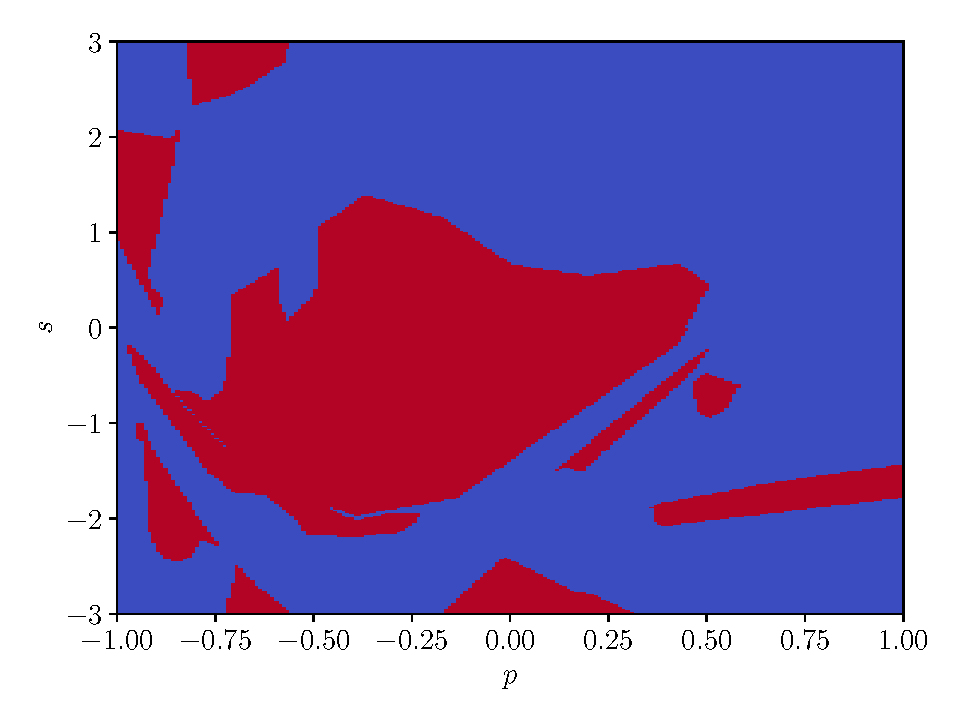
\includegraphics[width=\textwidth]{resources/pdf/5_mu_FQI.pdf}
            \caption{FQI}
        \end{subfigure}
        \hfill
        \begin{subfigure}{0.49\textwidth}
            \centering
            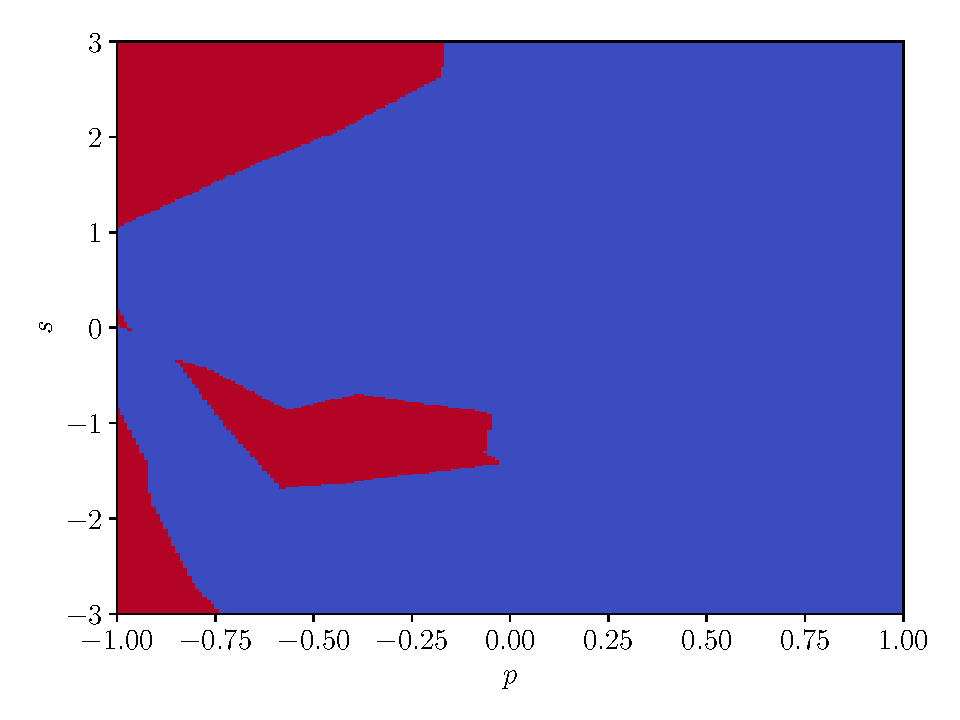
\includegraphics[width=\textwidth]{resources/pdf/5_mu_PQL_SGD.pdf}
            \caption{PQL (using SGD)}
        \end{subfigure}
        \noskipcaption{$\hat{\mu}^*$ policies inferred from $\hat{Q}$, for the FQI and PQL algorithms.}
        \label{fig:fqi.pql.sgd.mu}
    \end{figure}
    
    \begin{figure}[h]
        \centering
        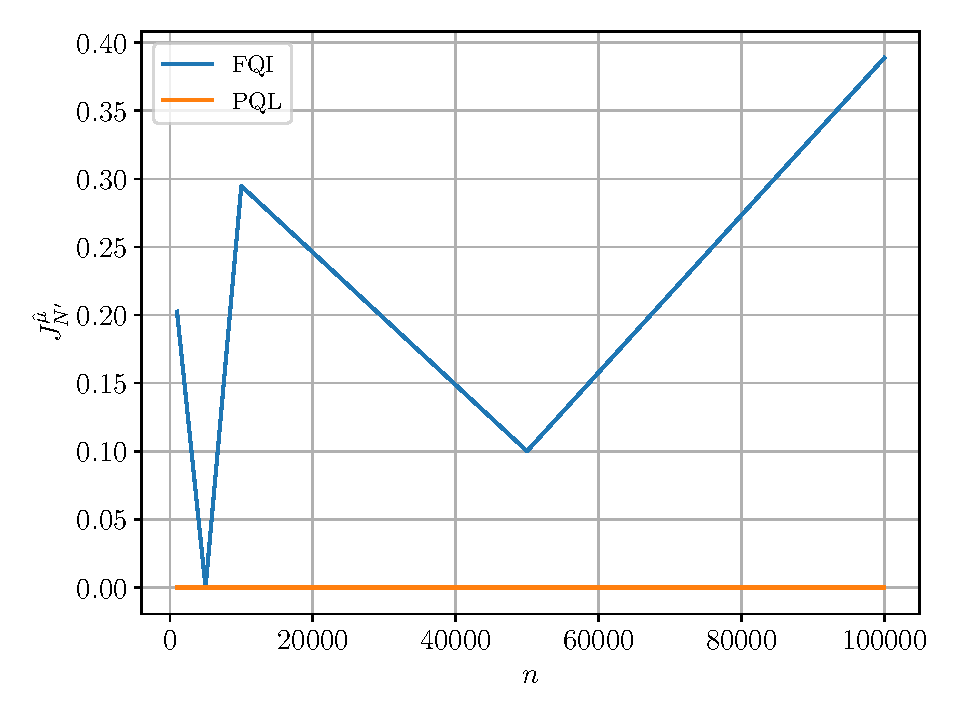
\includegraphics[width=0.6\textwidth]{resources/pdf/5_comparison_SGD.pdf}
        \caption{Expected return comparison between FQI and PQL algorithms.}
        \label{fig:fqi.pql.sgd.comparison}
    \end{figure}
    
    We can observe that the results, with the SGD optimizer, are terrible for the PQL algorithm, regardless of the size of the training set. Indeed, it didn't manage to find a good policy, while the FQI algorithm did, as expected from Section \ref{sec:fqi}. This is actually not surprising as \enquote{vanilla} PQL is known to perform poorly \cite{ernstinfo8003qfunctions}. Also, we note that FQI doesn't seem to improve consistently with the number of transitions in the training set, although the number of data points (5) is not sufficient to draw any conclusion.
    
    \subsubsection{Adam}
    
    Hoping to improve the quality of PQL's results, we replace the SGD optimizer by Adam \cite{kingma2014adam}. We also implement the \emph{Double Q-learning} (DQL) algorithm \cite{ernstinfo8003qfunctions}, which is a variant of the PQL algorithm where a target network is introduced. The results are presented in Figures \ref{fig:pql.dql.adam.mu} and \ref{fig:pql.dql.adam.comparison}.
    
    \begin{figure}[h]
        \centering
        \hfill
        \begin{subfigure}{0.49\textwidth}
            \centering
            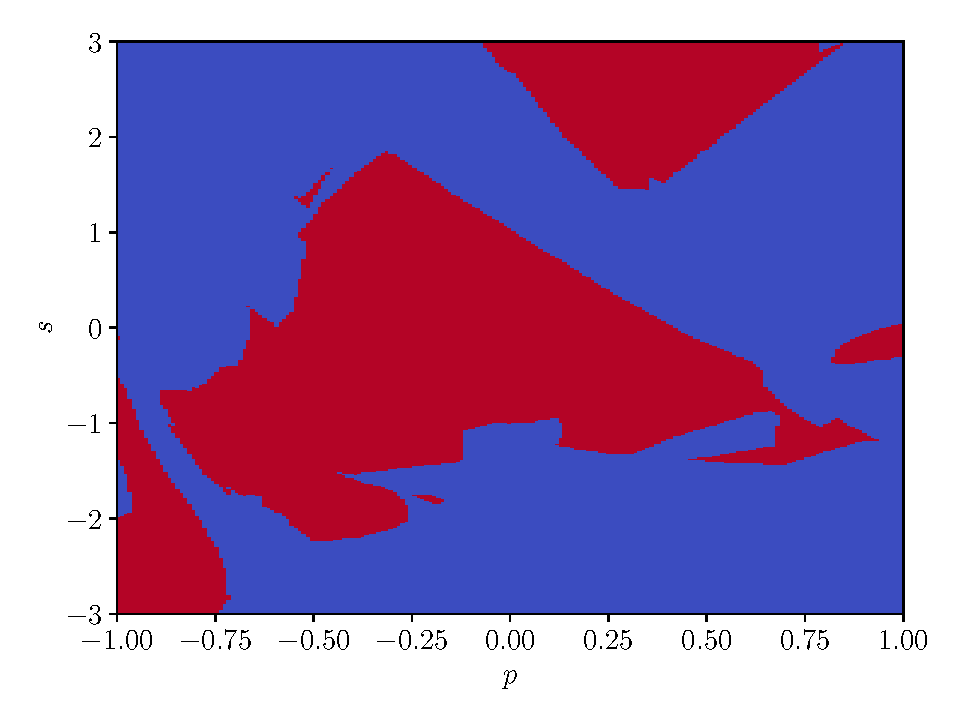
\includegraphics[width=\textwidth]{resources/pdf/5_mu_PQL_Adam.pdf}
            \caption{PQL}
        \end{subfigure}
        \hfill
        \begin{subfigure}{0.49\textwidth}
            \centering
            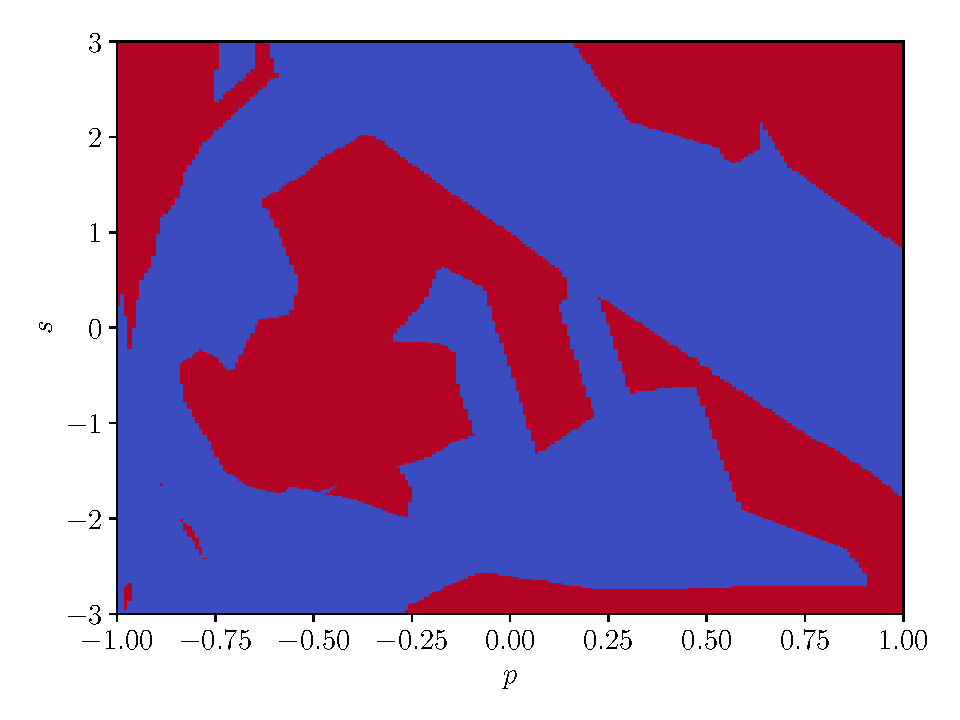
\includegraphics[width=\textwidth]{resources/pdf/5_mu_DQL_Adam.pdf}
            \caption{DQL}
        \end{subfigure}
        \noskipcaption{$\hat{\mu}^*$ policies inferred from $\hat{Q}$ for the PQL and DQL algorithms, using the Adam optimizer.}
        \label{fig:pql.dql.adam.mu}
    \end{figure}
    
    \begin{figure}[h]
        \centering
        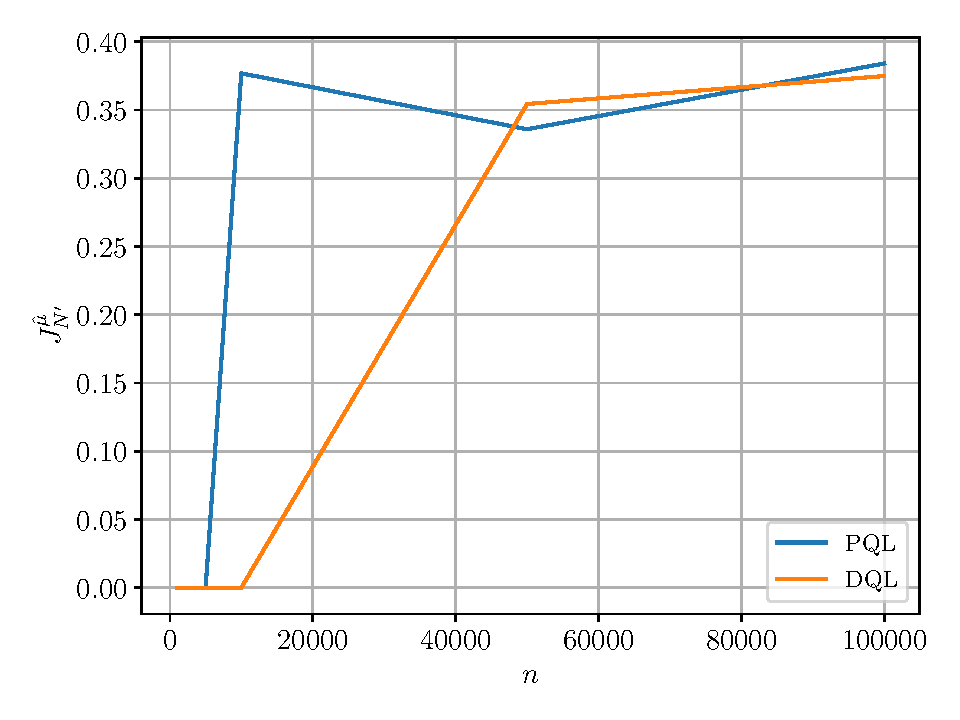
\includegraphics[width=0.6\textwidth]{resources/pdf/5_comparison_Adam.pdf}
        \caption{Expected return comparison between PQL and DQL algorithms, using the Adam optimizer.}
        \label{fig:pql.dql.adam.comparison}
    \end{figure}
    
    This time, the inferred policies are much closer to what they should be (\cf{} Figure \ref{fig:mu.xrt}), for both PQL and DQL. As a logical consequence, the expected returns are now almost matching those of FQI with the same MLP, although they still lag behind the Extremely Randomized Trees that reach \num{0.42} of expected return.
    
    Concerning convergence, it seems like PQL and DQL (with Adam) are more stable than FQI, but we should still keep in mind that we only have 5 data points and the experience was only conducted once. An improvement would have be to compute the mean and variance of the expected return while changing the random seeds, but it would take a lot of time.
    
    \newpage
    
    \section*{Normalised Parametric Q-Learning}
    
    To study the impact of normalisation, we divide the update term of the PQL algorithm by its 2-norm, \ie{} \eqref{eq:parametric.update} becomes
    \begin{equation}
        a \gets a + \alpha \frac{g}{\norm{g}_2}
    \end{equation}
    with
    \begin{equation*}
        g = \delta(x, u, r, x') \frac{\partial \hat{Q}(x, u, a)}{\partial a} ,
    \end{equation*}
    everything else remaining the same. The results are shown in Figures \ref{fig:parametric.q.learning.mu.normed} and \ref{fig:experimental.protocol.results.normed}.
    
    \begin{figure}[h]
        \centering
        \begin{subfigure}{0.49\textwidth}
            \centering
            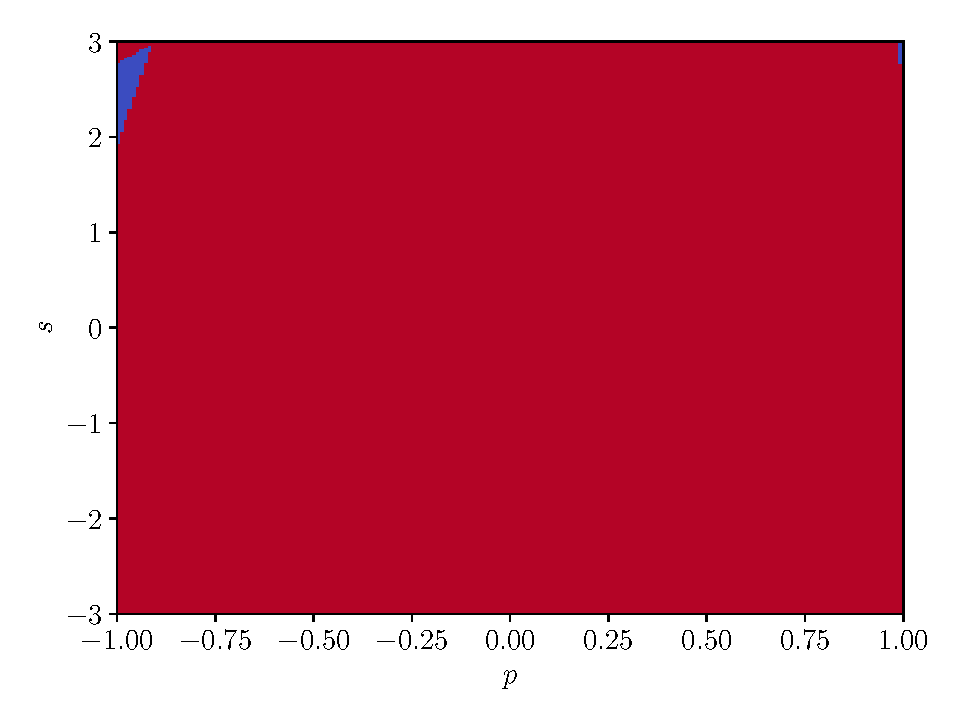
\includegraphics[width=\textwidth]{resources/pdf/5_mu_PQL_Adam_normed.pdf}
            \caption{PQL}
        \end{subfigure}
        \hfill
        \begin{subfigure}{0.49\textwidth}
            \centering
            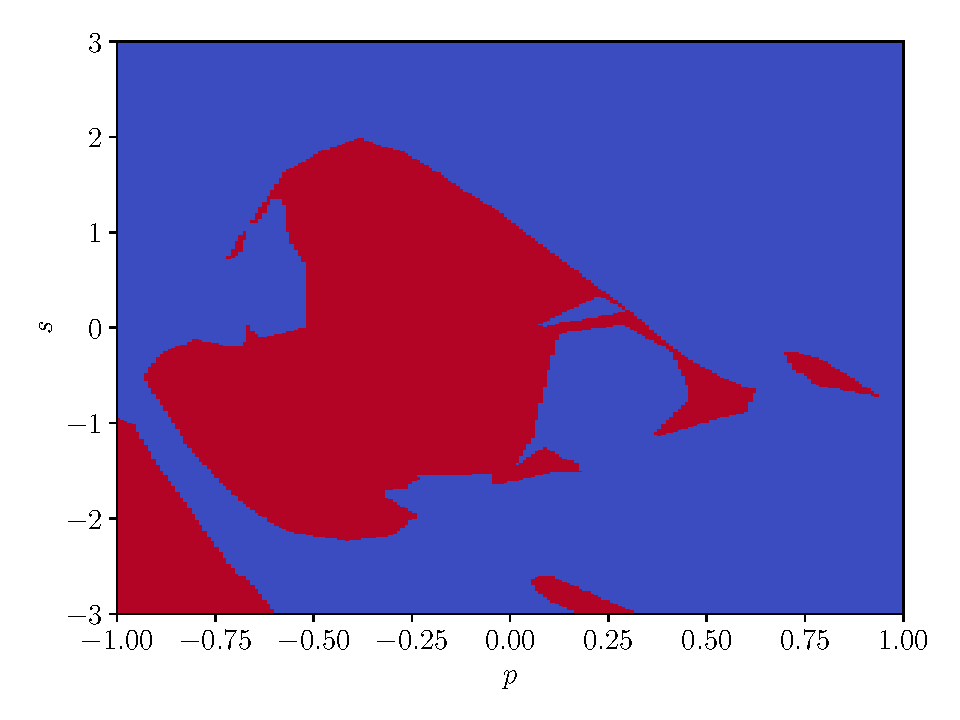
\includegraphics[width=\textwidth]{resources/pdf/5_mu_DQL_Adam_normed.pdf}
            \caption{DQL}
        \end{subfigure}
        \noskipcaption{$\hat{\mu}^*$ policies inferred from $\hat{Q}$ for the PQL and DQL algorithms, using the Adam optimizer and a normalised update term.}
        \label{fig:parametric.q.learning.mu.normed}
    \end{figure}
    
    \begin{figure}[h]
        \centering
        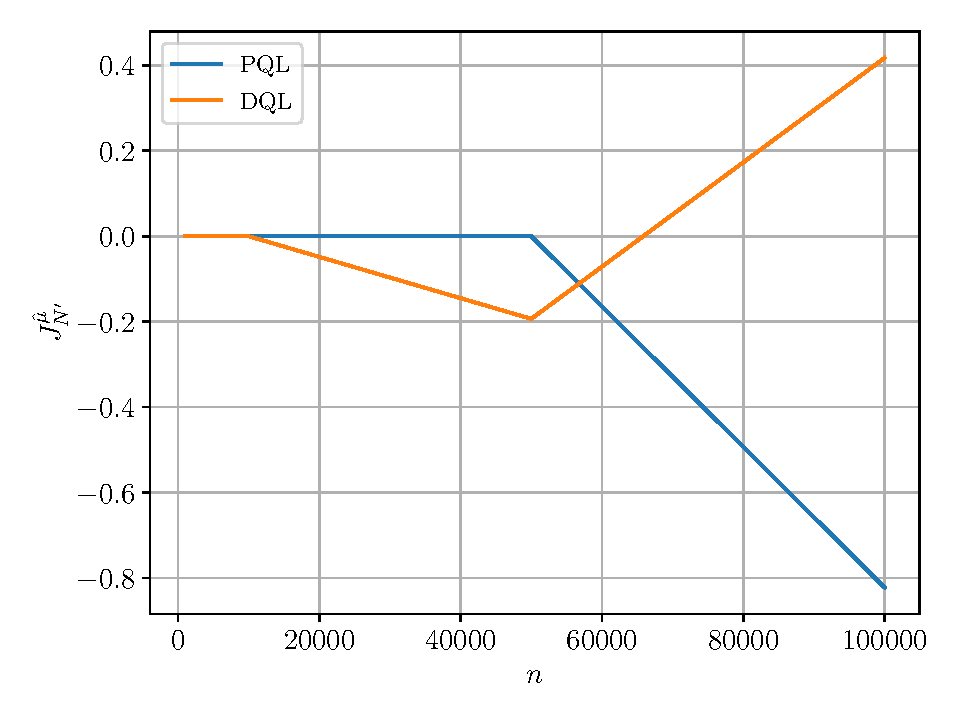
\includegraphics[width=0.6\textwidth]{resources/pdf/5_comparison_Adam_normed.pdf}
        \caption{Expected return comparison between PQL and DQL algorithms, using the Adam optimizer and a normalised update term.}
        \label{fig:experimental.protocol.results.normed}
    \end{figure}
    
    In this setting, the results are very different according to the algorithm. Indeed, normalised PQL provides a terrible (even worse than Linear Regression) policy, which is highlighted by its negative expected return, while DQL leads to a good (close \num{0.42}) expected return.
    
    However, for both algorithms, the policies change a lot depending on the number of one-step transitions in the training set $n$ (\cf{} Figure \ref{fig:experimental.protocol.results.normed}). Especially, PQL's expected return dropped inexplicably to \num{-0.8} for the largest set and DQL's expected return went from \num{-0.2} at $n = \num{50000}$ to \num{0.42} at $n = \num{100000}$.
    
    Because of this apparent instability, it is hard to draw any valuable conclusions. However, we investigated a bit and realized that, in our implementation, the update term's norm $\norm{g}_2$ is actually quite small (to the order of \num{e-2}). Therefore, normalizing $g$ actually increases it by a factor up to \num{e2}, since we didn't change the learning rate $\alpha$. This could explain the observed behaviours, as it is well known that having very large parameter updates lead to training instabilities.

    \newpage

    \printbibliography
\end{document}
